\documentclass[11pt]{article}


\usepackage[linesnumbered,ruled]{algorithm2e}
\SetKwRepeat{Do}{do}{while}
\usepackage[utf8]{inputenc}
\usepackage{amsmath,mathrsfs}
\usepackage{float}
\usepackage{amsfonts}
\usepackage{amssymb}
\usepackage{graphicx}
\usepackage{epstopdf}
\usepackage{caption}
\usepackage{listings}
\usepackage{url}
\usepackage{epstopdf}
\usepackage{subcaption}
\usepackage[left=2cm,right=2cm,top=1cm,bottom=1cm]{geometry}
\title{Assignment 2 Report}
\author{ Yue Hao, \url{yhao3@gmu.edu}}
\date{}

\newcommand{\lecture}[4]{\handout{#1}{#2}{#3}{#4}{#1}}

\newtheorem{theorem}{Theorem}
\newtheorem{corollary}[theorem]{Corollary}
\newtheorem{lemma}[theorem]{Lemma}
\newtheorem{observation}[theorem]{Observation}
\newtheorem{proposition}[theorem]{Proposition}
\newtheorem{definition}[theorem]{Definition}
\newtheorem{claim}[theorem]{Claim}
\newtheorem{fact}[theorem]{Fact}
\newtheorem{assumption}[theorem]{Assumption}

% 1-inch margins, from fullpage.sty by H.Partl, Version 2, Dec. 15, 1988.
\topmargin 0pt
\advance \topmargin by -\headheight
\advance \topmargin by -\headsep
\textheight 8.9in
\oddsidemargin 0pt
\evensidemargin \oddsidemargin
\marginparwidth 0.5in
\textwidth 6.5in

\parindent 0in
\parskip 1.5ex
%\renewcommand{\baselinestretch}{1.25}

\begin{document}

\maketitle

\section{Summary of the two methods}

Both methods use the same idea from paper \cite{secord}, however there are few major differences which can be summarized in Table \ref{tb:diff}.
\begin{table}[H]
\centering
\caption{Major Algorithmic Differences of the Two Methods}
\label{tb:diff}
\begin{tabular}{|c|c|c|}
\hline 
 & Hedcuter & Voronoi \\ 
\hline 
Initial Sites Distribution & Gaussian & Uniform \\ 
\hline 
Alg. for Voronoi & Image Propagation& Fortune\\ 
 \hline 
Cell Representation & Discretized Points & Polygon \\ 
\hline 
Metric of Displacement & Manhattan & Euclidean \\ 
\hline 
Disk Color & Cell Avg. Color & Controid Color \\ 
\hline 
Disk Radius & Cell Avg. Intensity & Cell Max Intensity\\ 
\hline
\end{tabular} 
\end{table}

\subsection{hedcuter method}
\begin{enumerate}

\item Centroidal Voronoi Tessellation (CVT)

The algorithm for generating CVT is summerized in  Algorithm \ref{alg:cvt_hed}.

Note there is an option in Algorithm \ref{alg:cvt_hed} Line 5, that the method can also use the maximum Manhattan distance as a metric for displacement besides the average.

Algorithm \ref{alg:sp_hed} shows that hedcuter collect $n$ points that randomly spreaded w.r.t. the intensity of greyscale image  as initial sites.

\begin{algorithm}[H]
    \SetKwInOut{Input}{Input}
    \SetKwInOut{Output}{Output}
    \SetKwFunction{Voronoi}{Voronoi}
    \SetKwFunction{Centroidal}{Centroidal}
    \SetKwFunction{SampleInitialPoints}{SampleInitialPoints}
    \Input{$I$: a grayscale image\\
    $n$: the number of points to be collected\\
    $d_t$: a user defined threshold for the average displacement}
    \Output{$C$: a collection of cells   representing the CVT\\
    	where $c.s$ is the 2D coordinate of site of cell $c$ in $C$\\
    	and $c.P$ is a collection of 2D coordinates marking the coverage of the cell}
    	   $C = \lbrace \rbrace$\\
    	$P$ = \SampleInitialPoints($I$,$n$)\\
   \Do{$d > d_t$} {
   	$V$ = \Voronoi($I$,$P$)\\
   	$P_c$ =  \Centroidal($I$,$V$)\\
   	$d =\frac{\sum_{p,p_c | p \in P, p_c \in P_c} {|p.x-p_c.x|+|p.y-p_c.y|}}{|P|} $\\
   	$P:=P_c$
   }
   \For {$p\in P$} {
      $c.s = p $\\
      $c.P = $ points in $V$ composing the cell that sited on $p$\\
      $C= C\cup  \lbrace c \rbrace$
   }   
      return $C$
    \caption{Centroidal\_Voronoi\_Tessellation($I$,$n$,$d_t$)}
        \label{alg:cvt_hed}
\end{algorithm}

\begin{algorithm}[H]
    \SetKwInOut{Input}{Input}
    \SetKwInOut{Output}{Output}
    \Input{$I$: a grayscale image w/ $I(p)$ being the intensity of pixel at $p$\\
    $n$: the number of points to be collected}
    \Output{$P$: a set of 2D coordinates of collected points}
    $P = \lbrace \rbrace $\\
   \While{$|P| < n$} {
   	$p$ = draw a coordinate uniformly random on image $I$ \\
   	$i$ = $I(p)$ \
   	$g$ = draw a random variable following a Gaussian distribution \\
   	\If{$i < g$} {
   	$P = P \cup p$
   	}
   }
      return $P$
    \caption{ SampleInitialPoints($I$,$n$)}
    \label{alg:sp_hed}
\end{algorithm}

\item Computing Voronoi Diagram

The method uses a image wave propagtion algorithm to calculate voronoi diagram which is summerized in  Algorithm \ref{alg:vor_hed}.


\begin{algorithm}[H]
    \SetKwInOut{Input}{Input}
    \SetKwInOut{Output}{Output}
    \SetKwFunction{ColorDist}{ColorDist}
    \Input{$P$: a set of 2D coordinates\\
    $I$: a grayscale image $I$ w/ $I(p)$ being the intensity pixel at $p$}
    \Output{$V$: a collection of cells representing the Voronoi Diagram,\\
    and $v.P$ is a collection of 2D coordinates marking the coverage of the cell
    }
    $H = \lbrace \rbrace$ (a heap data structure holding the points) \\
    $D = \lbrace \rbrace$ (an image sized contrainer) \\
    $R = \lbrace \rbrace$ (an image sized contrainer) \\
    \For {$p_i \in P$} {
    put $p_i$ in heap $H$ according to \ColorDist($I(p_i)$)\\
    $D(p_i)$ = \ColorDist($p_i$)\\
    $R(p_i)$ = $i$\\
    }
    \While {$H$ is not empty} {    
    $p$ = draw a point from the back of the heap $H$\\
    \For{each point $p_n$  neighboring $p$} {
    $d_n = D(p) + \ColorDist(p_n)$ \\
    	\If {$d_n < D(p)$ } {
    	$D(p_n) = d_n$\\
    	$R(p_n) = R(p)$\\
    	put $p_n$ in heap $H$ according to \ColorDist($I(p_n)$)
    	}
    }
    }
    
    \For {all points coordinates $p$ on image} {
    put all the points with the same $R(p)$ in the same voronoi cell $v_{R(p)}.P \in V$
    }
      return $V$
    \caption{Voronoi($I$,$P$)}
    \label{alg:vor_hed}
\end{algorithm}

\item Stippling

Finally, hedcuter method uses Algorithm \ref{alg:st_hed} to generate the stippling disks.

\begin{algorithm}[H]
    \SetKwInOut{Input}{Input}
    \SetKwInOut{Output}{Output}
    \Input{ $M$: an RGB color image  w/ $M(p)$ being the RGB color of pixel at $p$\\
    $I$: a grayscale image $I$ w/ $I(p)$ being the intensity pixel at $p$\\
    $C$: a collection of cells  representing the CVT\\
    	where $c.s$ is the 2D coordinate of site of cell $c$ in $C$\\
    	and $c.P$ is a collection of 2D coordinates marking the coverage of the cell}
    \Output{$D$: a collection of disks of the Stipples\\
    where $d.c$ is the 2D coordinates of the center of $d$ in $D$, \\
     $d.rgb$ is the RGB color and $d.r$ is the radius
    }
    $D = \lbrace \rbrace $\\
    \For {$c \in C$} {
    $d.c = c.s$\\
    $d.rgb =\frac{\sum_{p \in c.P} {M(p)} } {|c.P|}$ \\
    $i = \frac{\sum_{p \in c.P} {I(p)} } {|c.P|}$ \\
    $d.r = \frac{100*r}{i+100}$ where $r$ is a default constant\\
     $D = D \cup \lbrace d \rbrace$
    }
      return $D$
    \caption{Create\_Disks($M$,$I$,$C$)}
    \label{alg:st_hed}
\end{algorithm}

\end{enumerate}

\subsection{voronoi method}

\begin{enumerate}

\item Centroidal Voronoi Tessellation (CVT)


The algorithm for generating CVT is summerized in  Algorithm \ref{alg:cvt_vor}, which is very similar  to the one in hedcuter methods, the only difference are the cell representation, methods to create initial samplings, and distance metric.

Algorithm \ref{alg:sp_vor} shows that hedcuter collect $n$ points that randomly spreaded w.r.t. the intensity of greyscale image  as initial sites.

\begin{algorithm}[H]
    \SetKwInOut{Input}{Input}
    \SetKwInOut{Output}{Output}
    \SetKwFunction{VoronoiFortune}{VoronoiFortune}
    \SetKwFunction{Centroidal}{Centroidal}
    \SetKwFunction{CreateInitialDistribution}{CreateInitialDistribution}
    \Input{$I$: a grayscale image\\
    $n$: the number of points to be collected\\
    $d_t$: a user defined threshold for the average displacement}
    \Output{$C$: a collection of cells   representing the CVT\\
    	where $c.s$ is the 2D coordinate of site of cell $c$ in $C$\\
    	and $c.V$ is a collection of 2D coordinates marking the boundary of the cell\\
    	and $c.E$ is a collection of edges marking the  boundary of the cell}
    	     $C = \lbrace \rbrace$\\
    	$P$ = \CreateInitialDistribution($I$,$n$)\\
   \Do{$d > d_t$} {
   	$V$ = \VoronoiFortune($I$,$P$)\\
   	$P_c$ =  \Centroidal($I$,$V$)\\
   	$d =\frac{\sum_{p,p_c | p \in P, p_c \in P_c} {\sqrt{(p.x-p_c.x)^2+(p.y-p_c.y)^2}}}{|P|} $\\
   	$P:=P_c$
   }
   \For {$p\in P$} {
      $c.s = p $\\
      $c.V = $ points in $V$ bounding the cell that sited on $p$\\
      $c.E = $ edges in $V$ bounding the cell that sited on $p$\\
      $C= C\cup  \lbrace c \rbrace$
   }   
      return $C$
    \caption{Centroidal\_Voronoi\_Tessellation($I$,$n$,$d_t$)}
        \label{alg:cvt_vor}
\end{algorithm}



\begin{algorithm}[H]
    \SetKwInOut{Input}{Input}
    \SetKwInOut{Output}{Output}
    \Input{$I$: a grayscale image w/ $I(p)$ being the intensity of pixel at $p$\\
    $n$: the number of points to be collected}
    \Output{$P$: a set of 2D coordinates of collected points}
    $P = \lbrace \rbrace $\\
   \While{$|P| < n$} {
   	$p$ = draw a coordinate uniformly random on image $I$ \\
   	$i$ = $I(p)$ \
   	$g$ = draw a random variable uniformly random \\
   	\If{$i < g$} {
   	$P = P \cup p$
   	}
   }
      return $P$
    \caption{ CreateInitialDistribution($I$,$n$)}
    \label{alg:sp_vor}
\end{algorithm}

\item Computing Voronoi Diagram

This method uses the Fortune's algorithm which was fully discussed in lecture. For the sake of brevity, the pseudocode is neglected here.

\item Stippling

The stippling technique is very similar to hedcuter method, where only minor difference is the color of disk is solely determined on the controid's color (shown in Alg. \ref{alg:st_vor} Line 4), slightly different handling of radius  (shown in Alg. \ref{alg:st_vor} Line 6-7).

\begin{algorithm}[H]
    \SetKwInOut{Input}{Input}
    \SetKwInOut{Output}{Output}
    \Input{ $M$: an RGB color image  w/ $M(p)$ being the RGB color of pixel at $p$\\
    $I$: a grayscale image $I$ w/ $M(p)$ being the intensity pixel at $p$\\
    $C$: a collection of cells   representing the CVT\\
    	where $c.s$ is the 2D coordinate of site of cell $c$ in $C$\\
    	and $c.V$ is a collection of 2D coordinates marking the boundary of the cell\\
    	and $c.E$ is a collection of edges marking the  boundary of the cell}
    \Output{$D$: a collection of disks of the Stipples\\
    where $d.c$ is the 2D coordinates of the center of $d$ in $D$, \\
     $d.rgb$ is the RGB color and $d.r$ is the radius
    }
    $D = \lbrace \rbrace $\\
    \For {$c \in C$} {
    $d.c = c.s$\\
    $d.rgb =M(c.s)$ \\
    $P$ = sampling points in $c$\\
    $i = \sum_{p \in P} {I(p)}$ \\
    $d.r =r*\frac{i}{max(i \text{ for all } c \in C)}$ where $r$ is a default constant\\
     $D = D \cup \lbrace d \rbrace$
    }
      return $D$
    \caption{Stippling($M$,$I$,$C$)}
    \label{alg:st_vor}
\end{algorithm}

\end{enumerate}

\section{Comparison of the two methods}
Unless otherwise specified, all the output in this section are using the following settings for both methods in Table \ref{tb:param}, these parameters are tunes for the purpose of unifying the output for both algorithms (shown in question 1), and used as baseline for comparison the output with various parameters/input adjusted in the remaining questions.
\begin{table}[H]
\centering
\caption{Baseline Parameters }
\label{tb:param}
\begin{tabular}{|c|c|c|}
\hline 
 & Hedcuter & Voronoi \\ 
\hline 
Num of points & 1000 & 1000 \\ 
\hline 
Threshold of Displacement& 1.0 & 0.14\\ 
 \hline 
Default Radius & 7 & 0,7 \\ 
\hline 
Color & Black & Black \\ 
\hline 
Sub-pixels & 1 & 5 \\ 
\hline 
\end{tabular} 
\end{table}
For the hedcuter, GPU is NOT used and max iteration is set to $\infty$.

\begin{enumerate}
\item Do you get the same results by running the same program on the same image multiple times?

\begin{figure}[H]
    \centering
        \begin{subfigure}{0.4\textwidth}
        \centering
        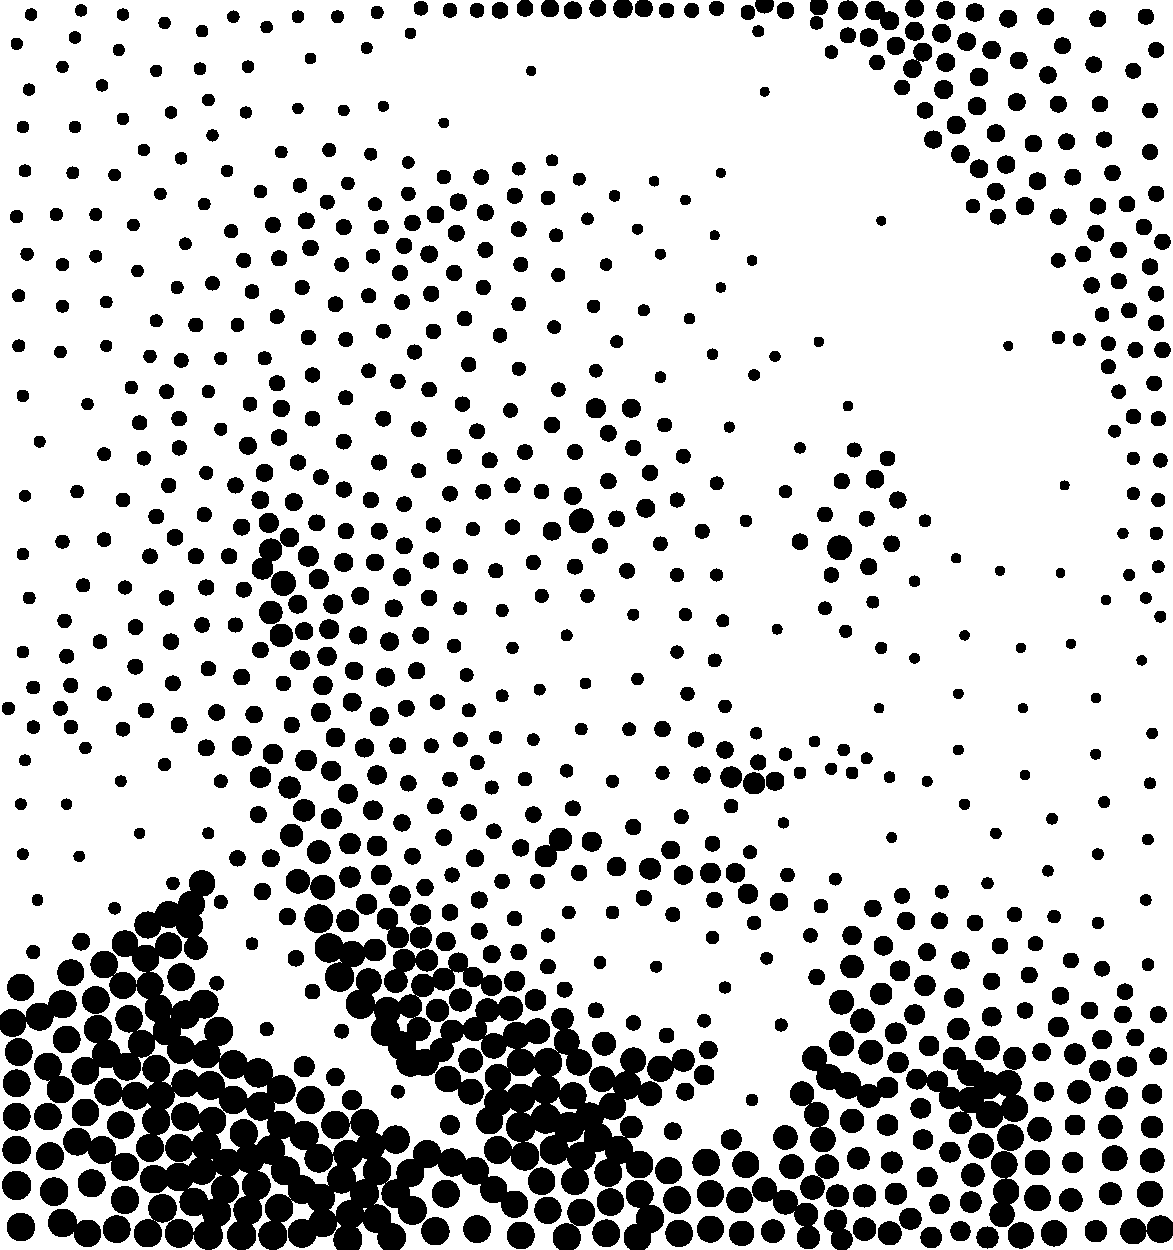
\includegraphics[width=\textwidth]{../results/hedcuter/1-1.pdf}
        \caption{1st run}
    \end{subfigure}
    \begin{subfigure}{0.4\textwidth}
        \centering
        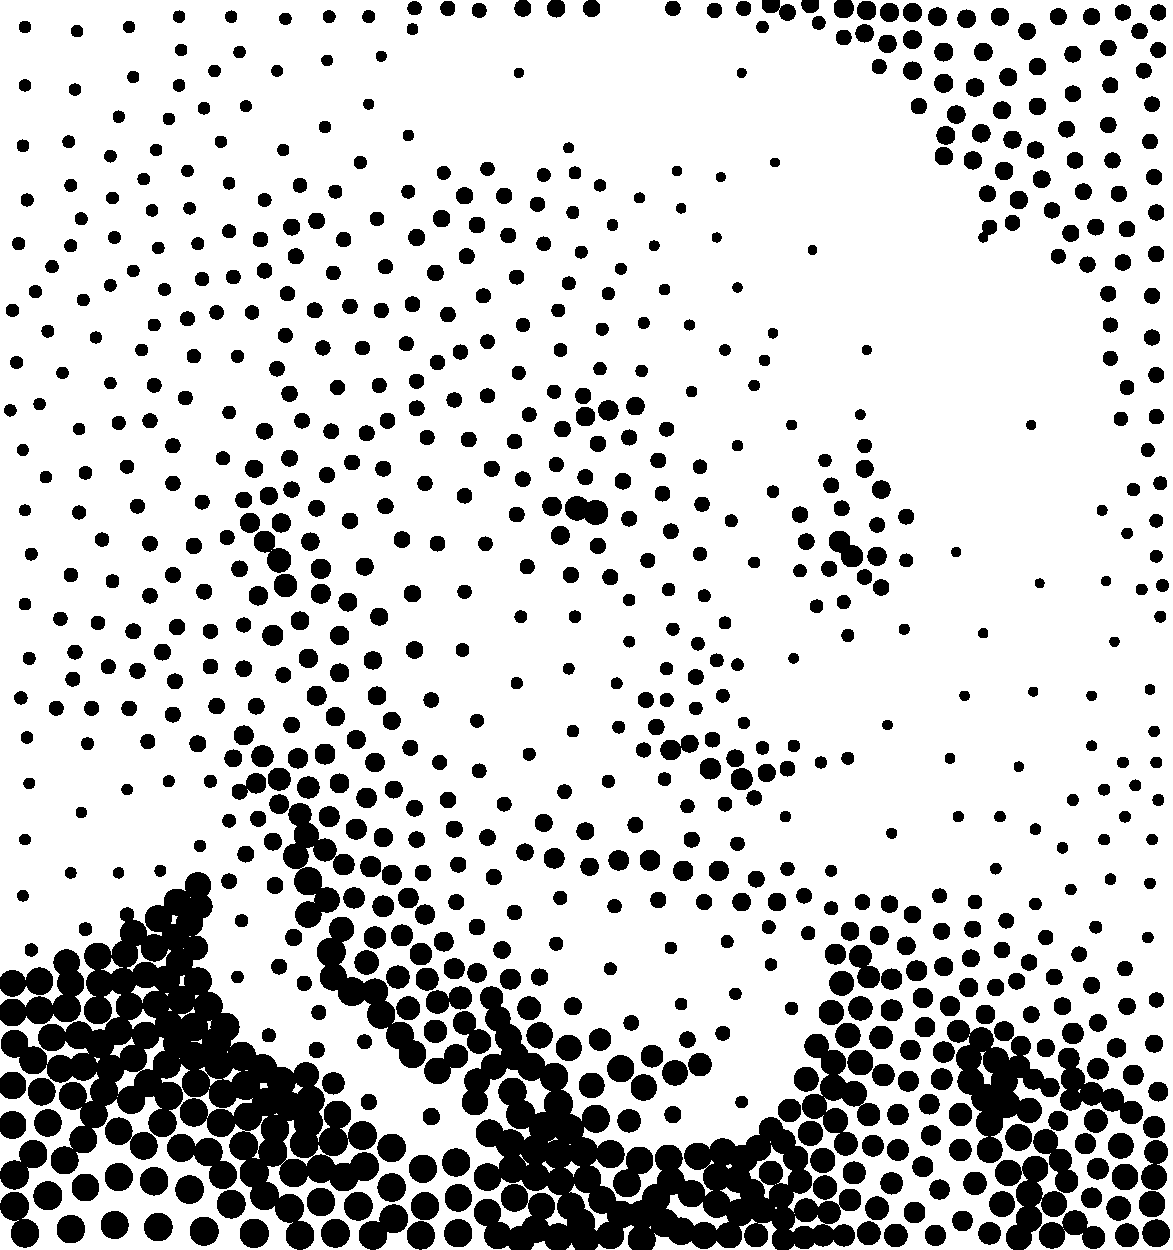
\includegraphics[width=\textwidth]{../results/hedcuter/1-2.pdf}
        \caption{2nd run}
    \end{subfigure}
    \label{fig:1}
    \caption{Hedcuter}
\end{figure}

\begin{figure}[H]
    \centering
        \begin{subfigure}{0.4\textwidth}
        \centering
        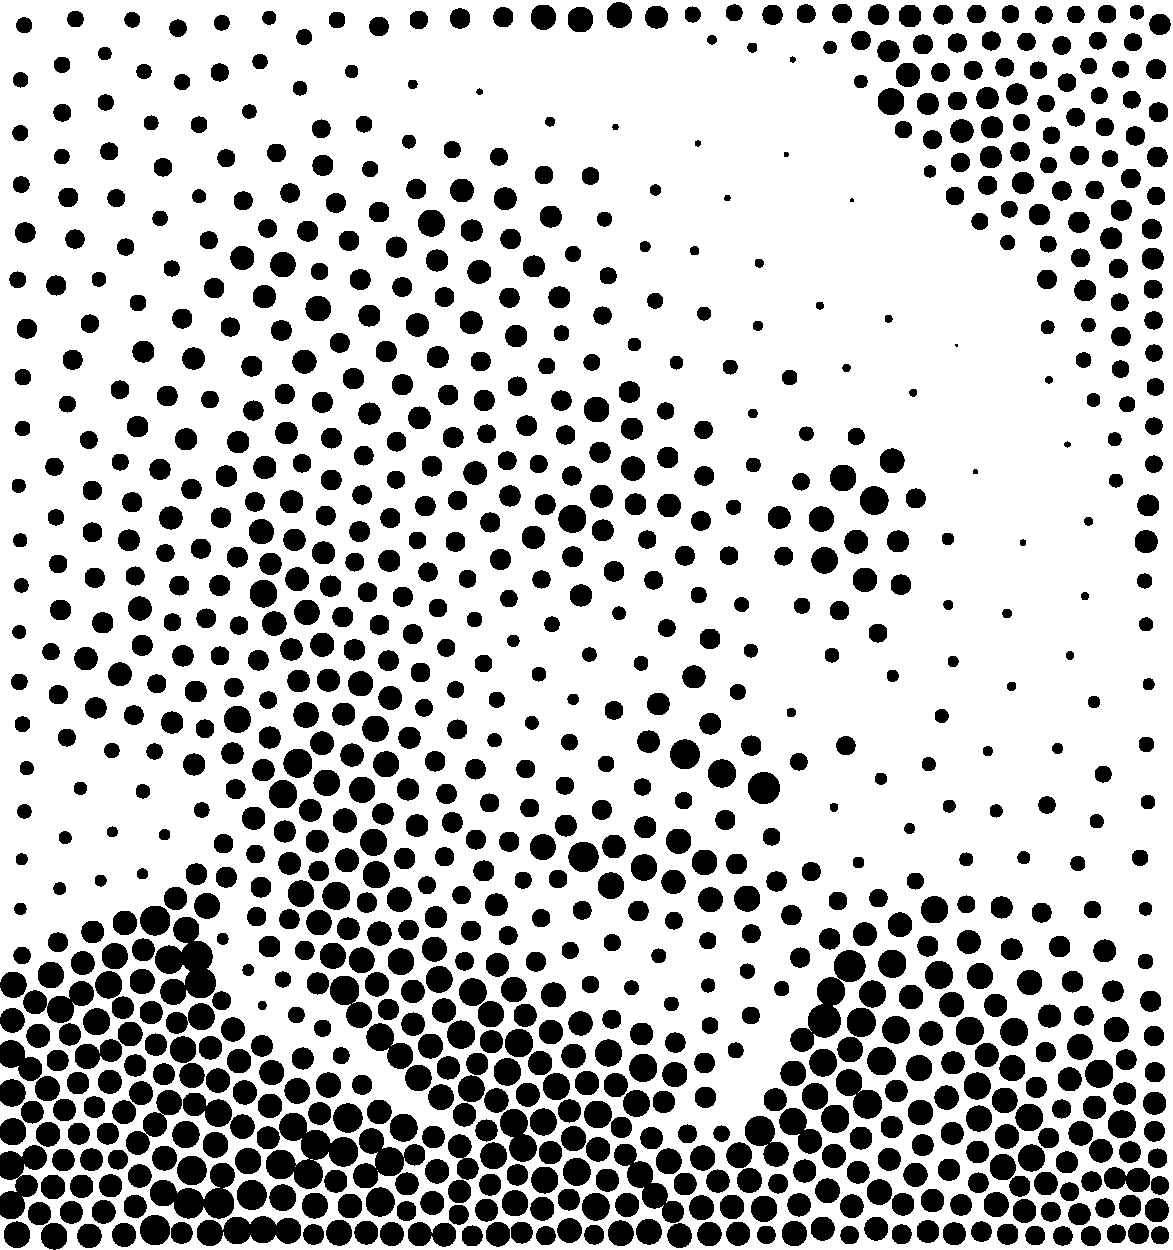
\includegraphics[width=\textwidth]{../results/voronoi/1-1.pdf}
    \caption{1st run}
    \end{subfigure}
    \begin{subfigure}{0.4\textwidth}
        \centering
        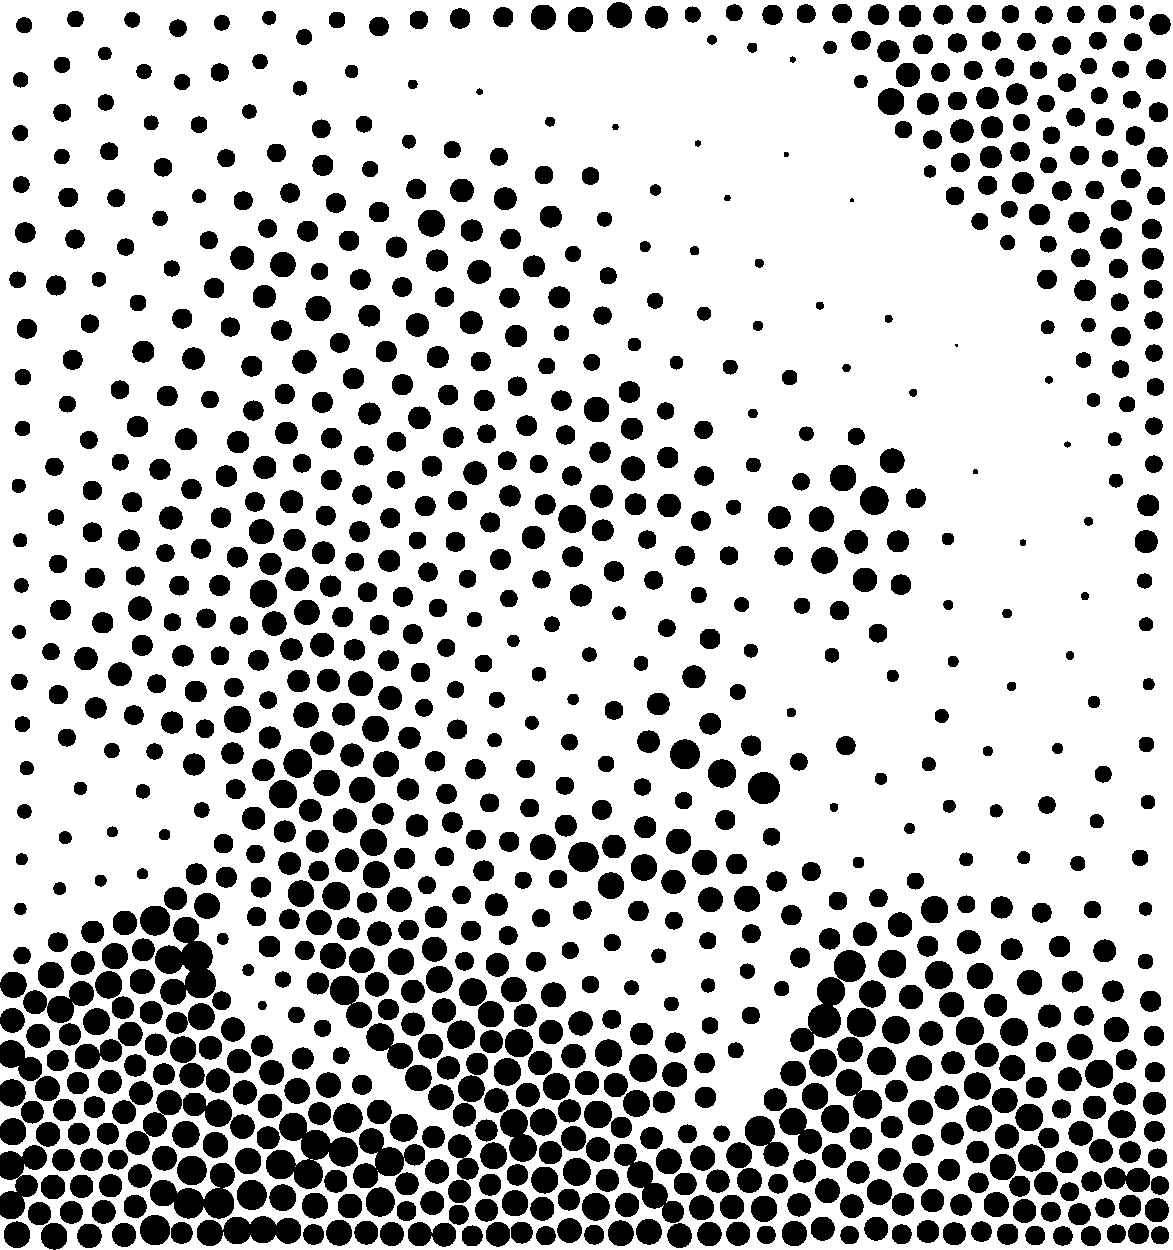
\includegraphics[width=\textwidth]{../results/voronoi/1-2.pdf}
         \caption{2nd run}
    \end{subfigure}
    \label{fig:2}
      \caption{Voronoi}
\end{figure}

I do NOT get the same results running hedcuter on the same image, due the the randomness introduced when sampling the initial sites.

I do get the same results running voronoi. Although the initial sites are also generated randomly, the random seed that  voronoi uses is \textit{boost::mt19937}, which creates a  pseudo-random number generator. A numbers the random number produced will be the same every time the program is run.


\item If you vary the number of the disks in the output images, do these implementations produce the same distribution in the final image? If not, why?

\begin{figure}[H]
    \centering
        \begin{subfigure}{0.4\textwidth}
        \centering
        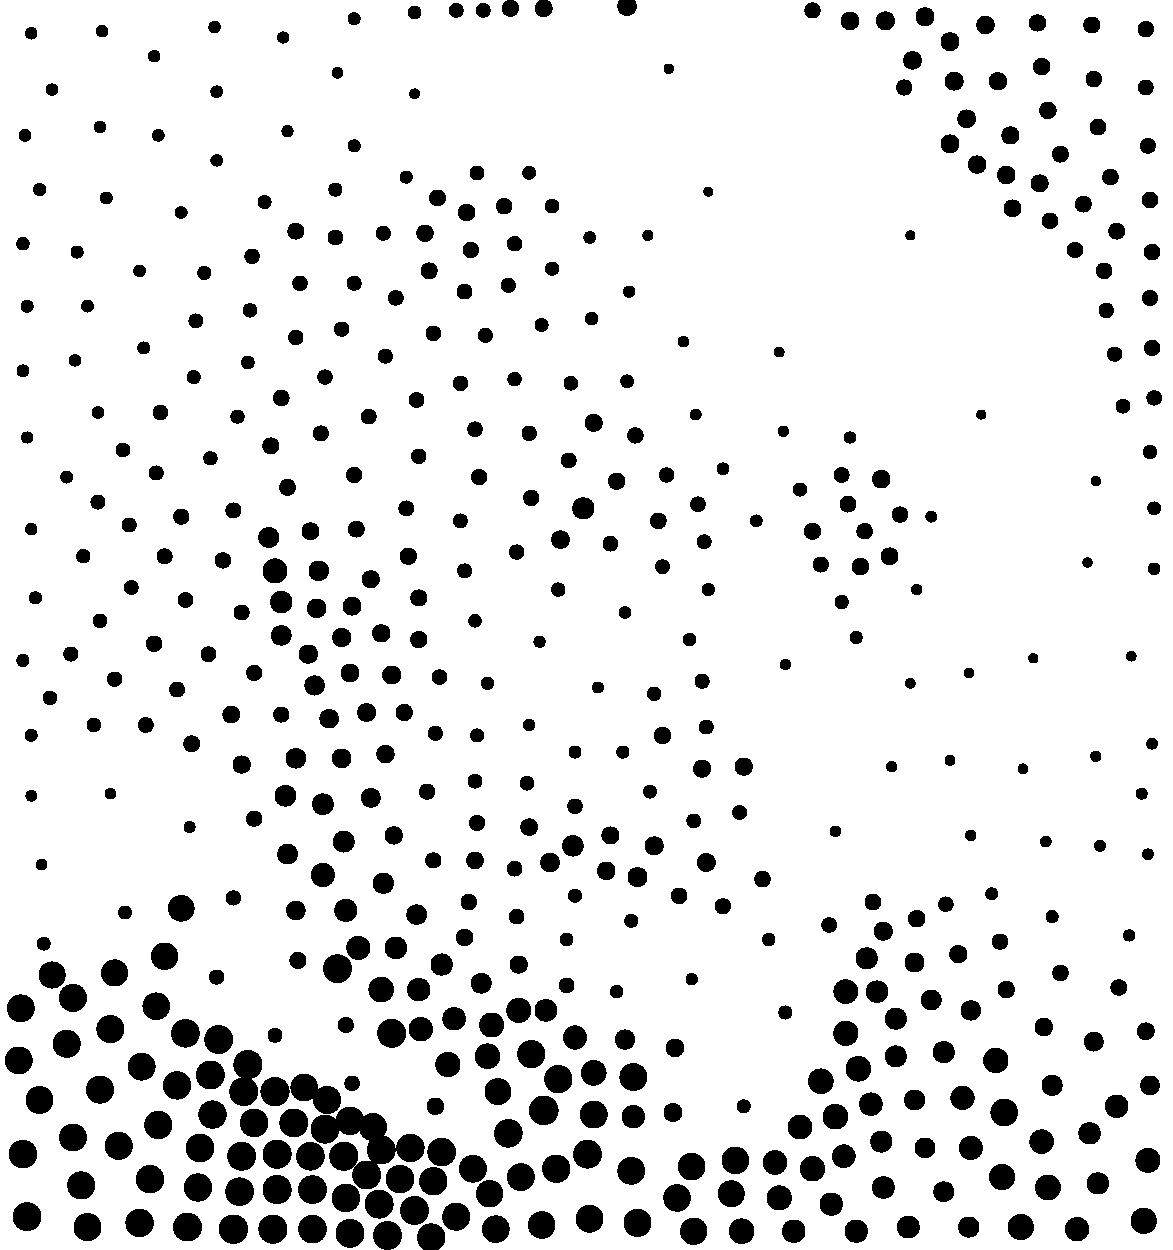
\includegraphics[width=\textwidth]{../results/hedcuter/2-1.pdf}
         \caption{500 disks}
    \end{subfigure}
    \begin{subfigure}{0.4\textwidth}
        \centering
        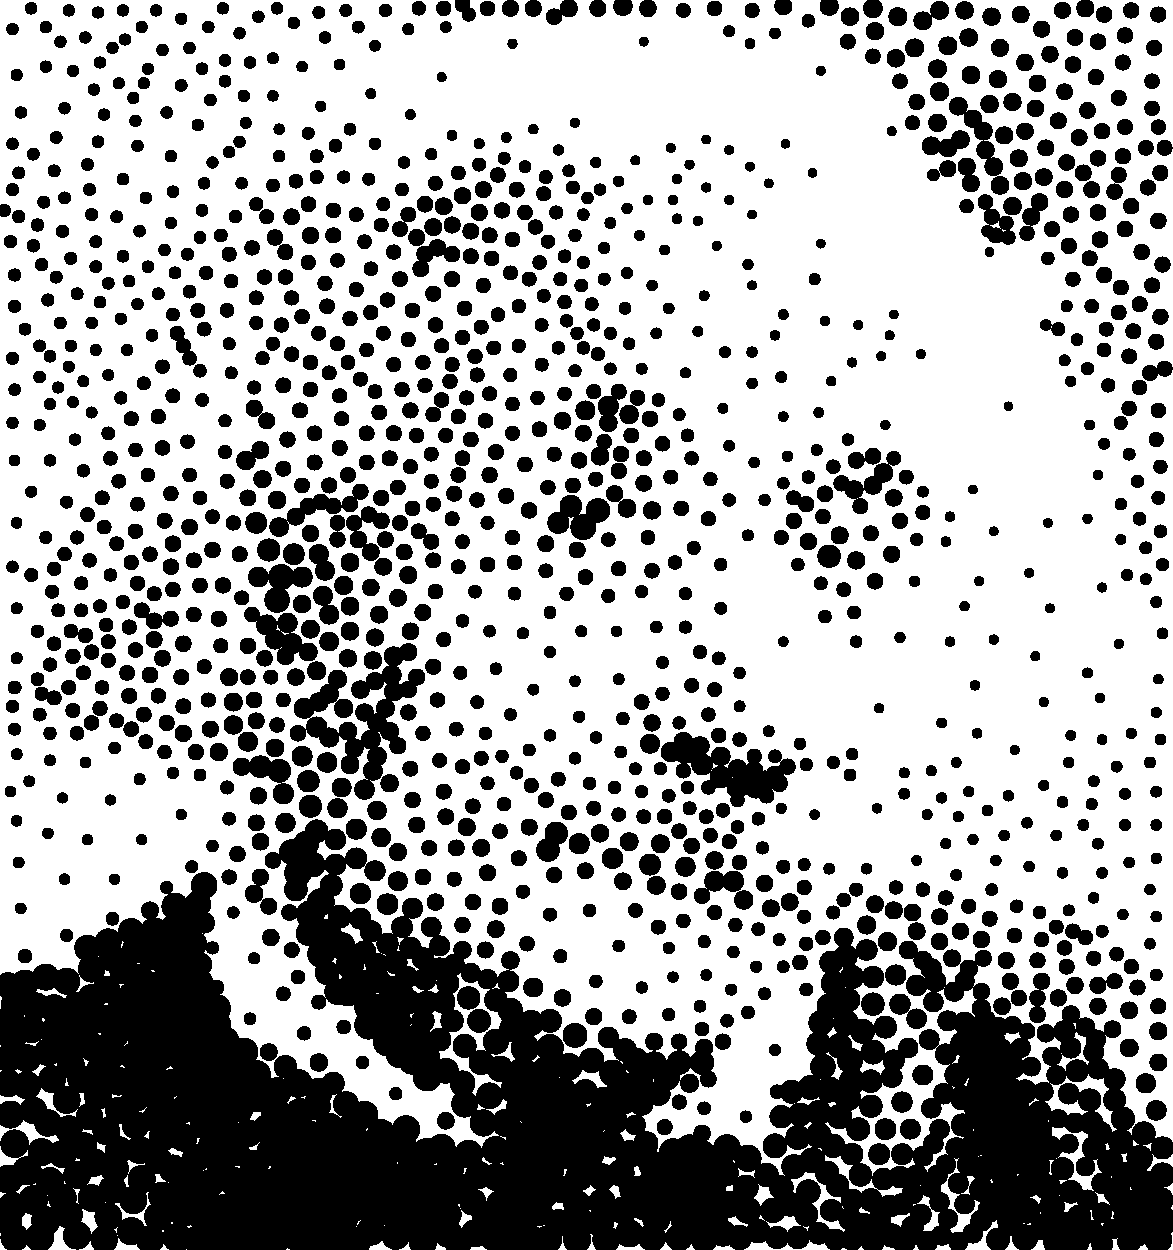
\includegraphics[width=\textwidth]{../results/hedcuter/2-2.pdf}
         \caption{2000 disks}
    \end{subfigure}
    \label{fig:1}
        \caption{Hedcuter}
\end{figure}

\begin{figure}[H]
    \centering
        \begin{subfigure}{0.4\textwidth}
        \centering
        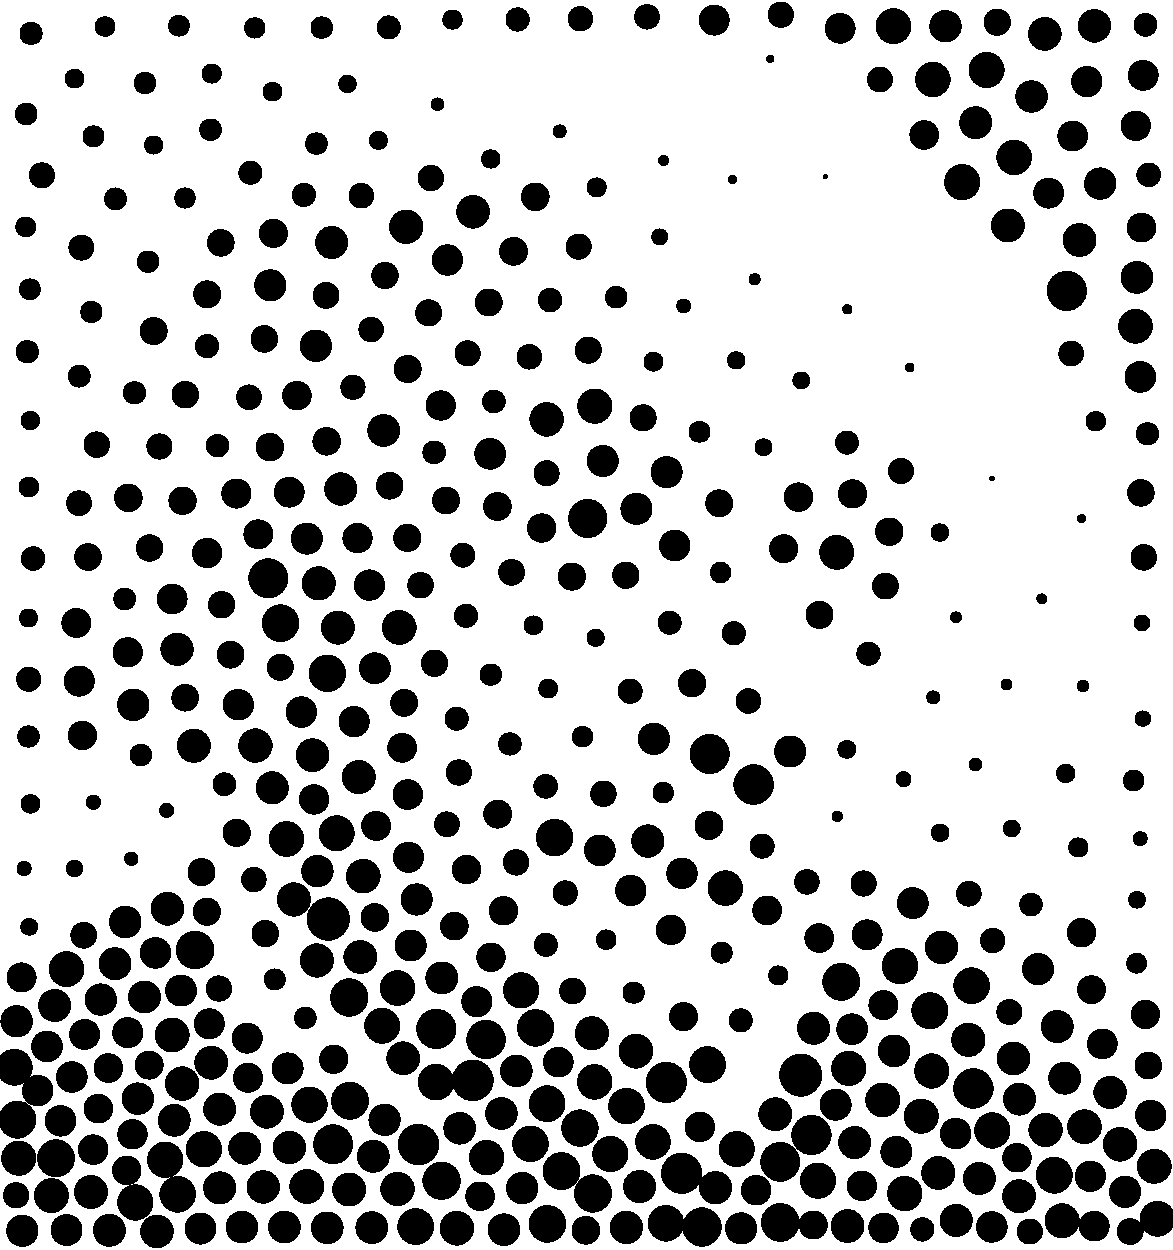
\includegraphics[width=\textwidth]{../results/voronoi/2-1.pdf}
 \caption{500 disks}
    \end{subfigure}
    \begin{subfigure}{0.4\textwidth}
        \centering
        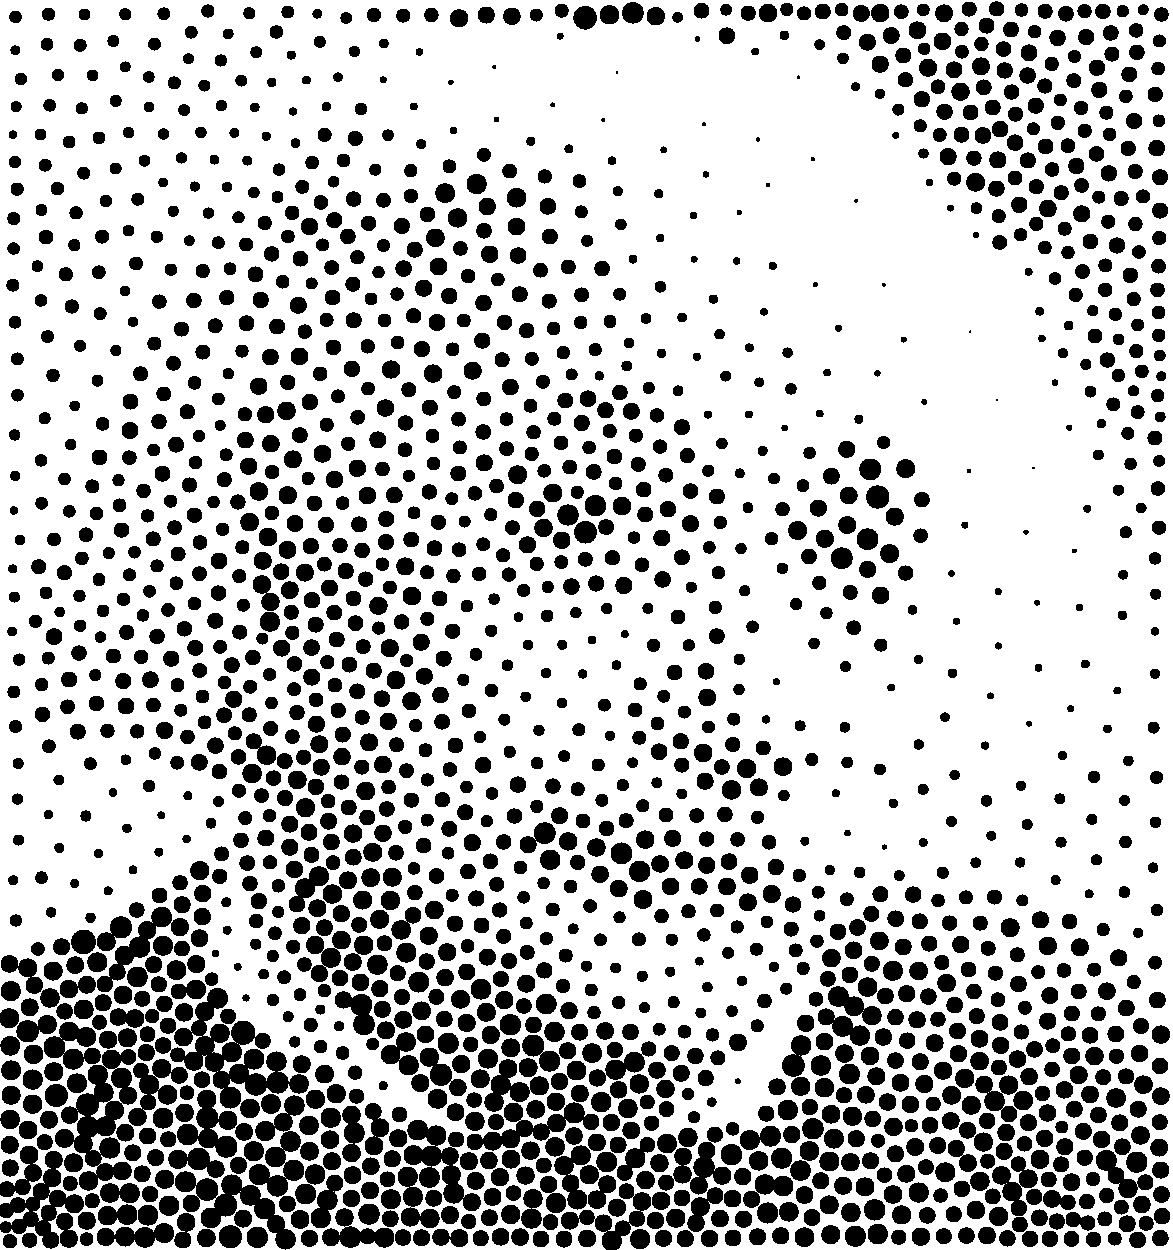
\includegraphics[width=\textwidth]{../results/voronoi/2-2.pdf}
 \caption{2000 disks}
    \end{subfigure}
    \caption{Voronoi}
    \label{fig:2}
\end{figure}

The disk distributions are different between hedcuter and voronoi, as  hedcuter biases on darker region based on a Gaussian distribution, while voronoi is more of an uniform distribution. Vary the number of disks does not affect the distribution among both algorithm themselves as the distribution of random sampling is independent of how many samples your use.

\item If you vary the number of the disks in the output images, is a method faster than the other?

\begin{figure}[H]
    \centering
        \begin{subfigure}{0.45\textwidth}
        \centering
        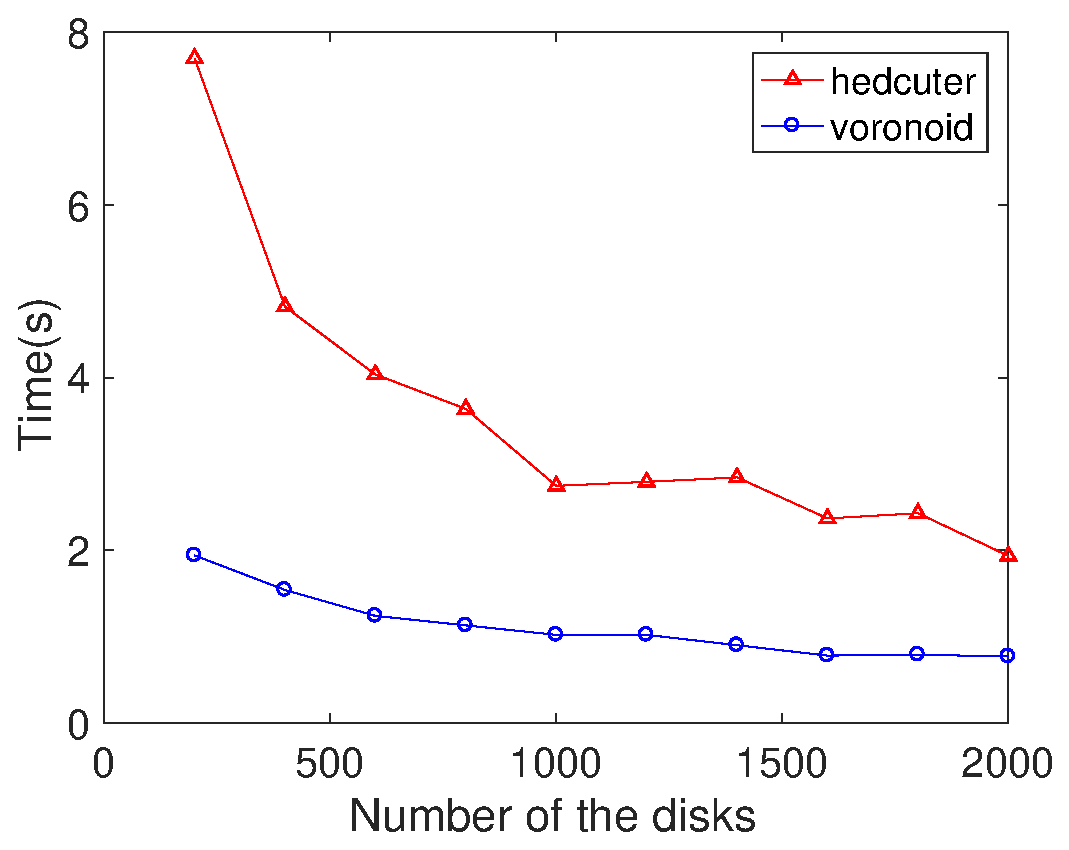
\includegraphics[width=\textwidth]{figs/time2.eps}
    \caption{Threshold: hedcuter = 1, voronoi = 0.5}
    \end{subfigure}
    \begin{subfigure}{0.45\textwidth}
        \centering
        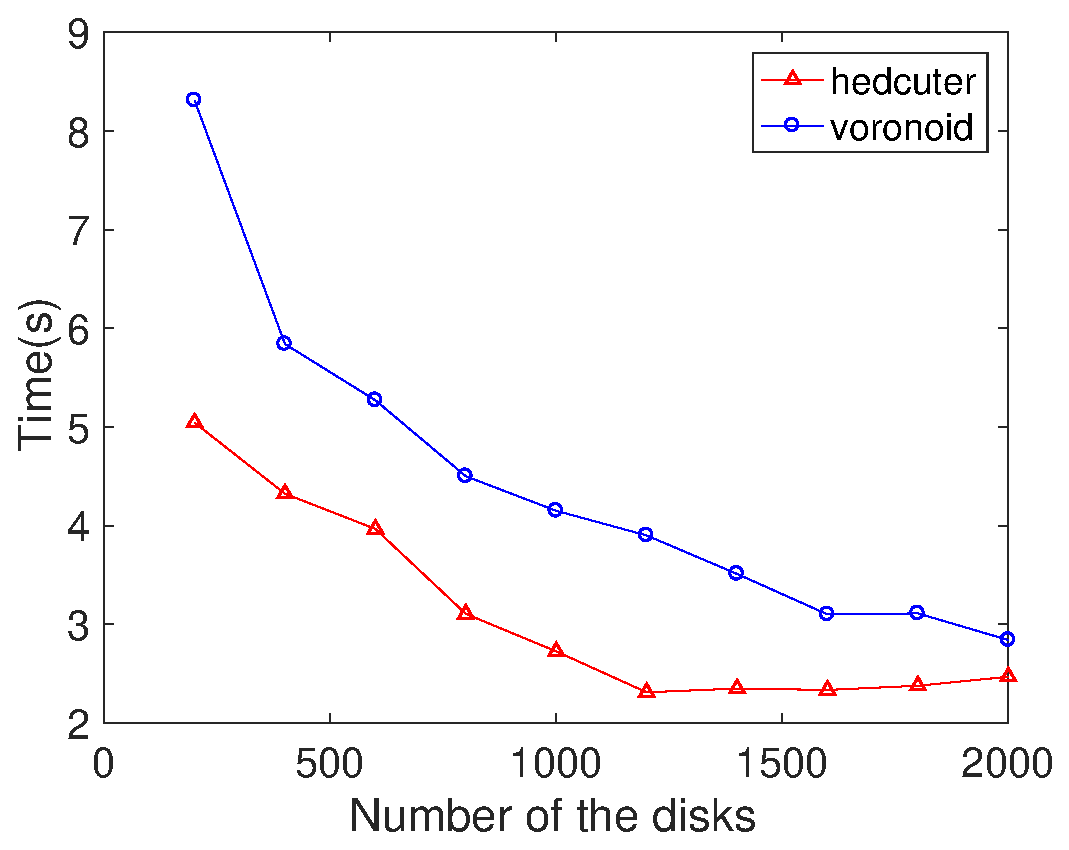
\includegraphics[width=\textwidth]{figs/time.eps}
         \caption{Threshold: hedcuter = 1, voronoi  = 0.14 }
    \end{subfigure}
    \label{fig:2}
      \caption{Running time vs number of disks.}
\end{figure}

No method is strictly superior to the other in terms of running time. As it depends on other parameters besides the number of disks. However, both methods seem to require less time to converge for larger number of disks.

\item Does the size (number of pixels), image brightness or contrast of image increase or decrease their difference?

\begin{figure}[H]
    \centering
        \begin{subfigure}{0.4\textwidth}
        \centering
        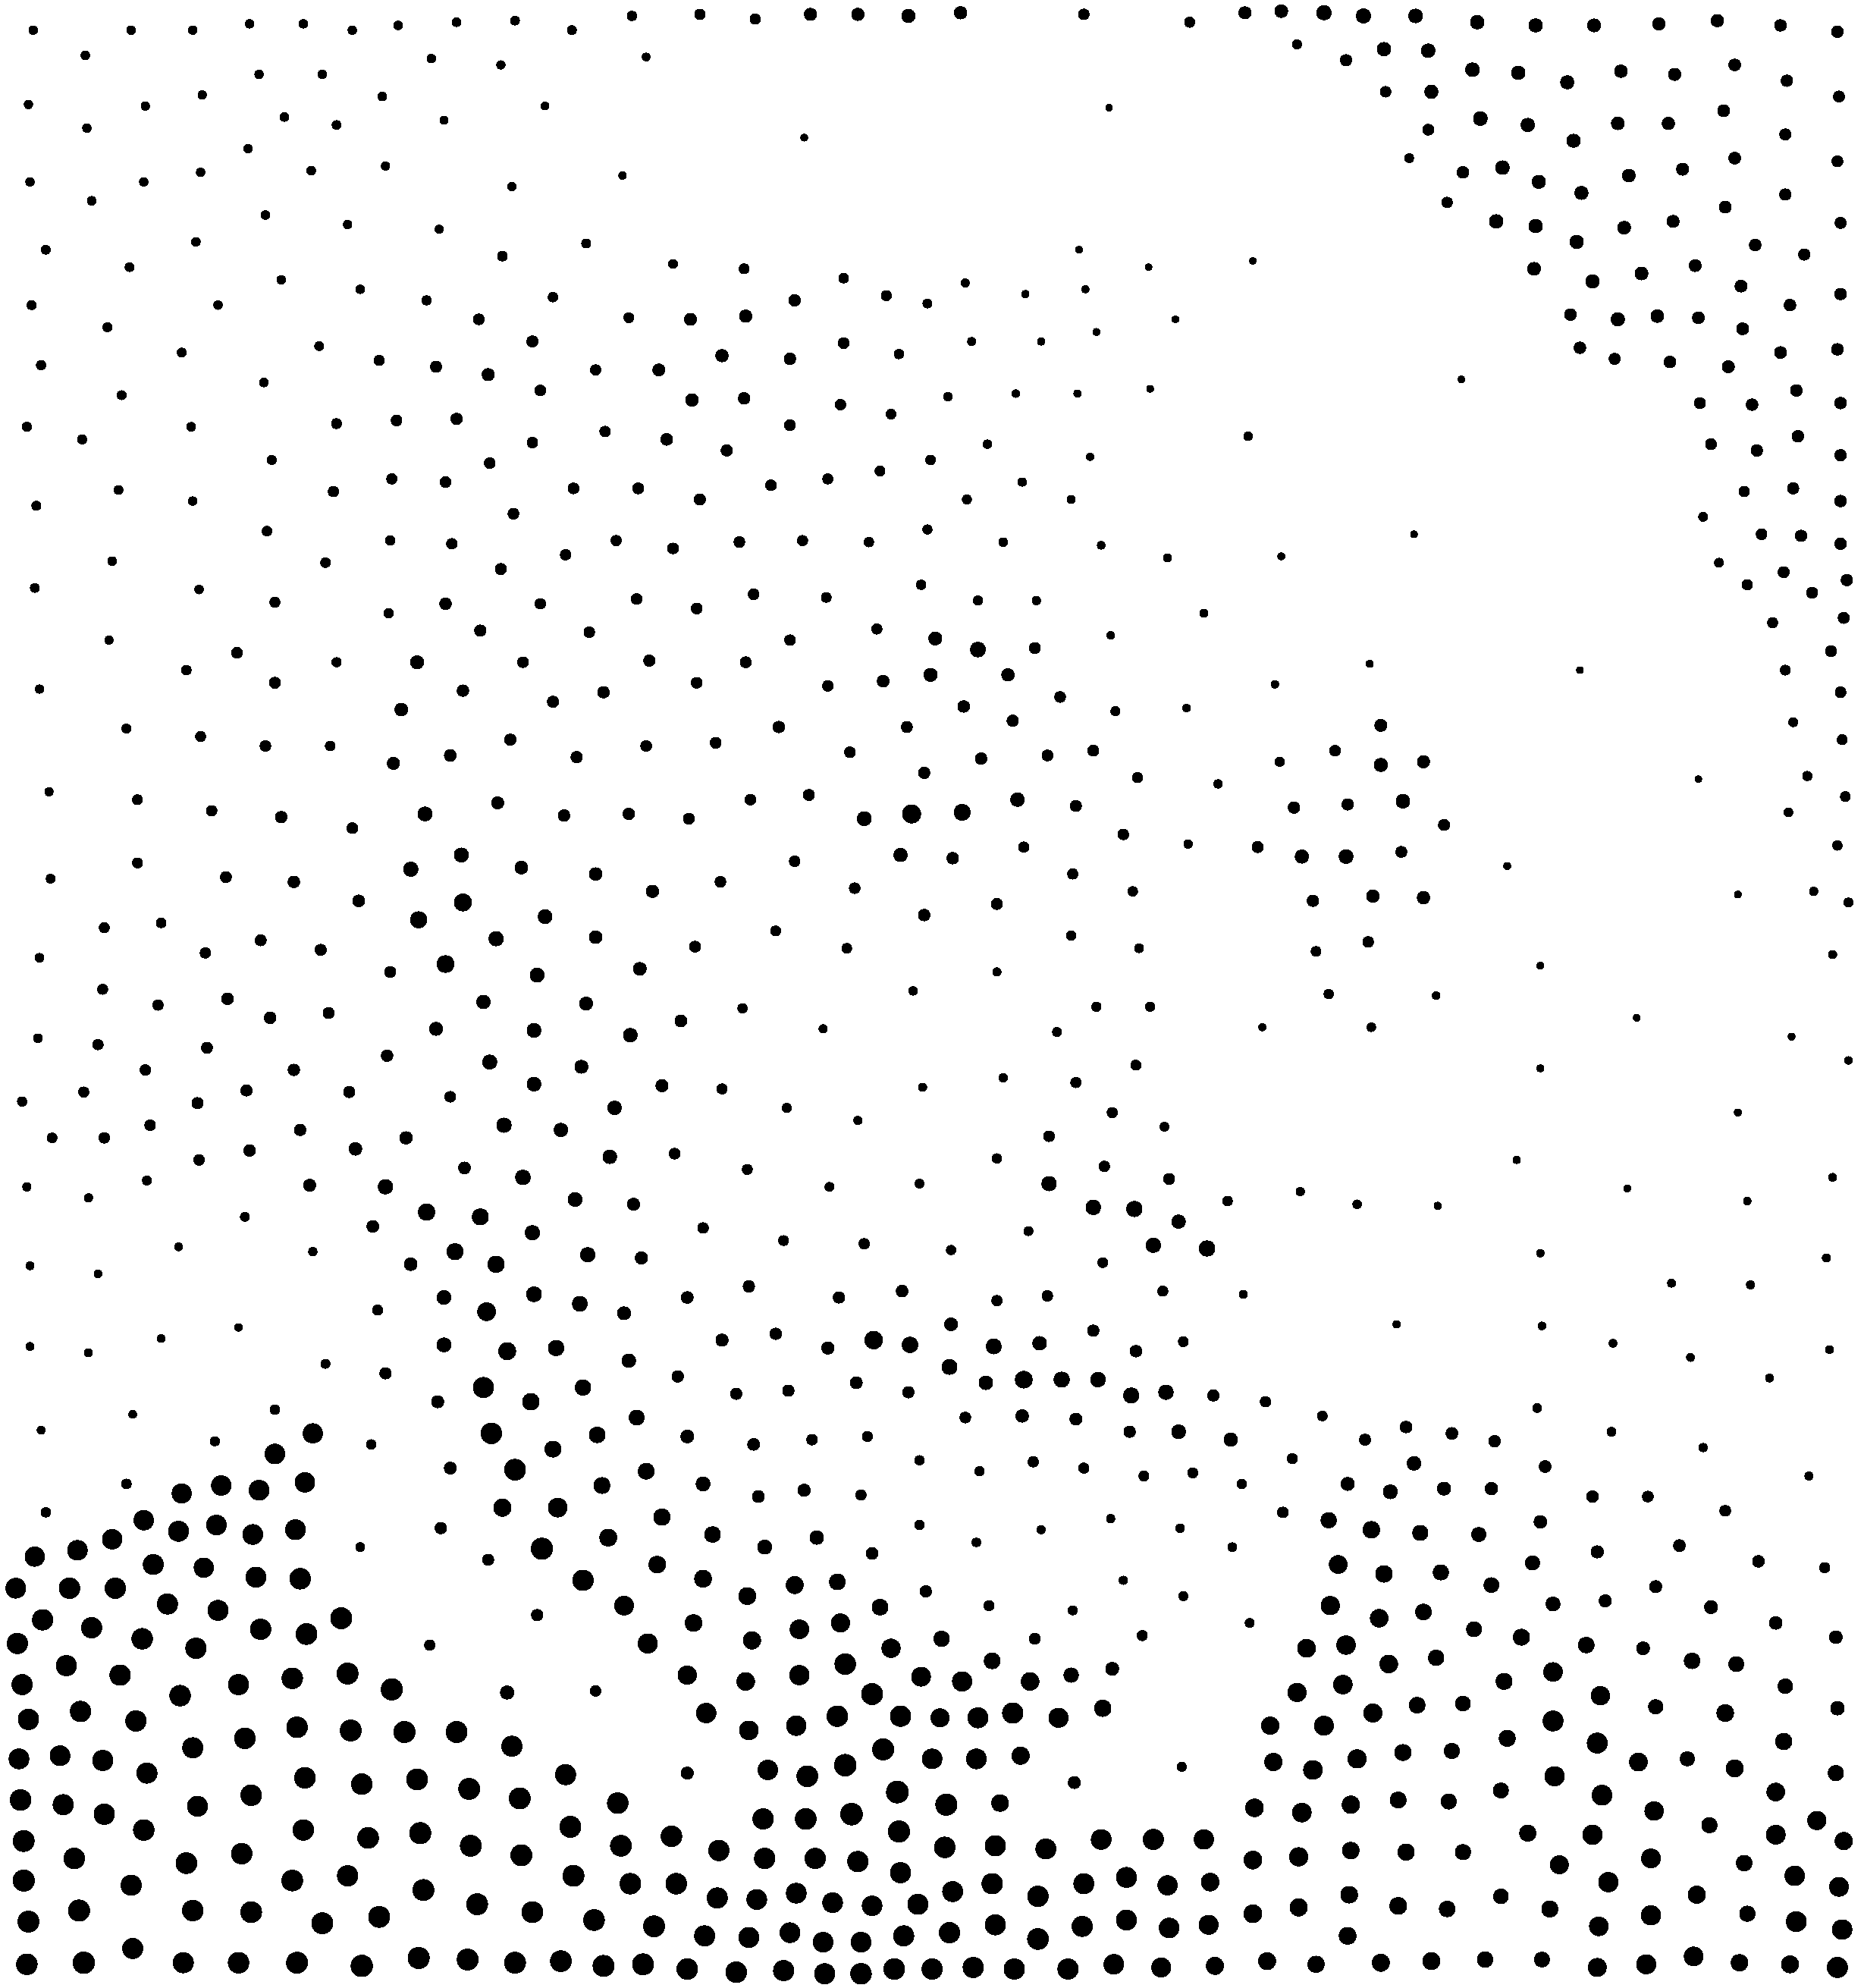
\includegraphics[width=\textwidth]{../results/hedcuter/3-5.pdf}
         \caption{Large image size}
    \end{subfigure}
    \begin{subfigure}{0.4\textwidth}
        \centering
        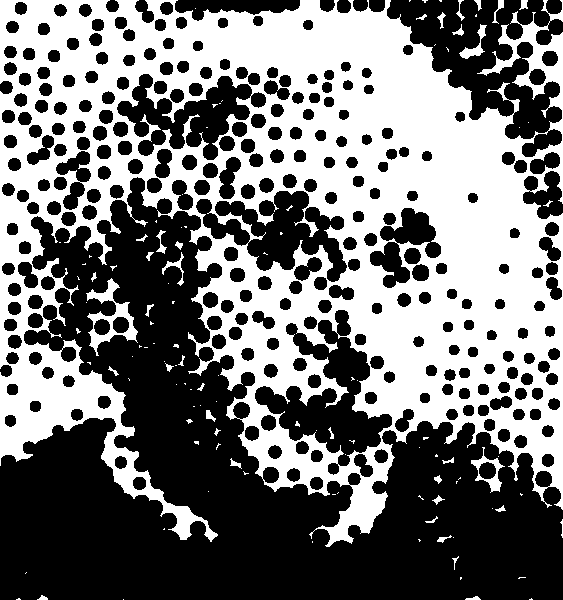
\includegraphics[width=\textwidth]{../results/hedcuter/3-6.pdf}
         \caption{Small image size}
    \end{subfigure}
    \label{fig:1}
        \caption{Hedcuter}
\end{figure}

\begin{figure}[H]
    \centering
        \begin{subfigure}{0.4\textwidth}
        \centering
        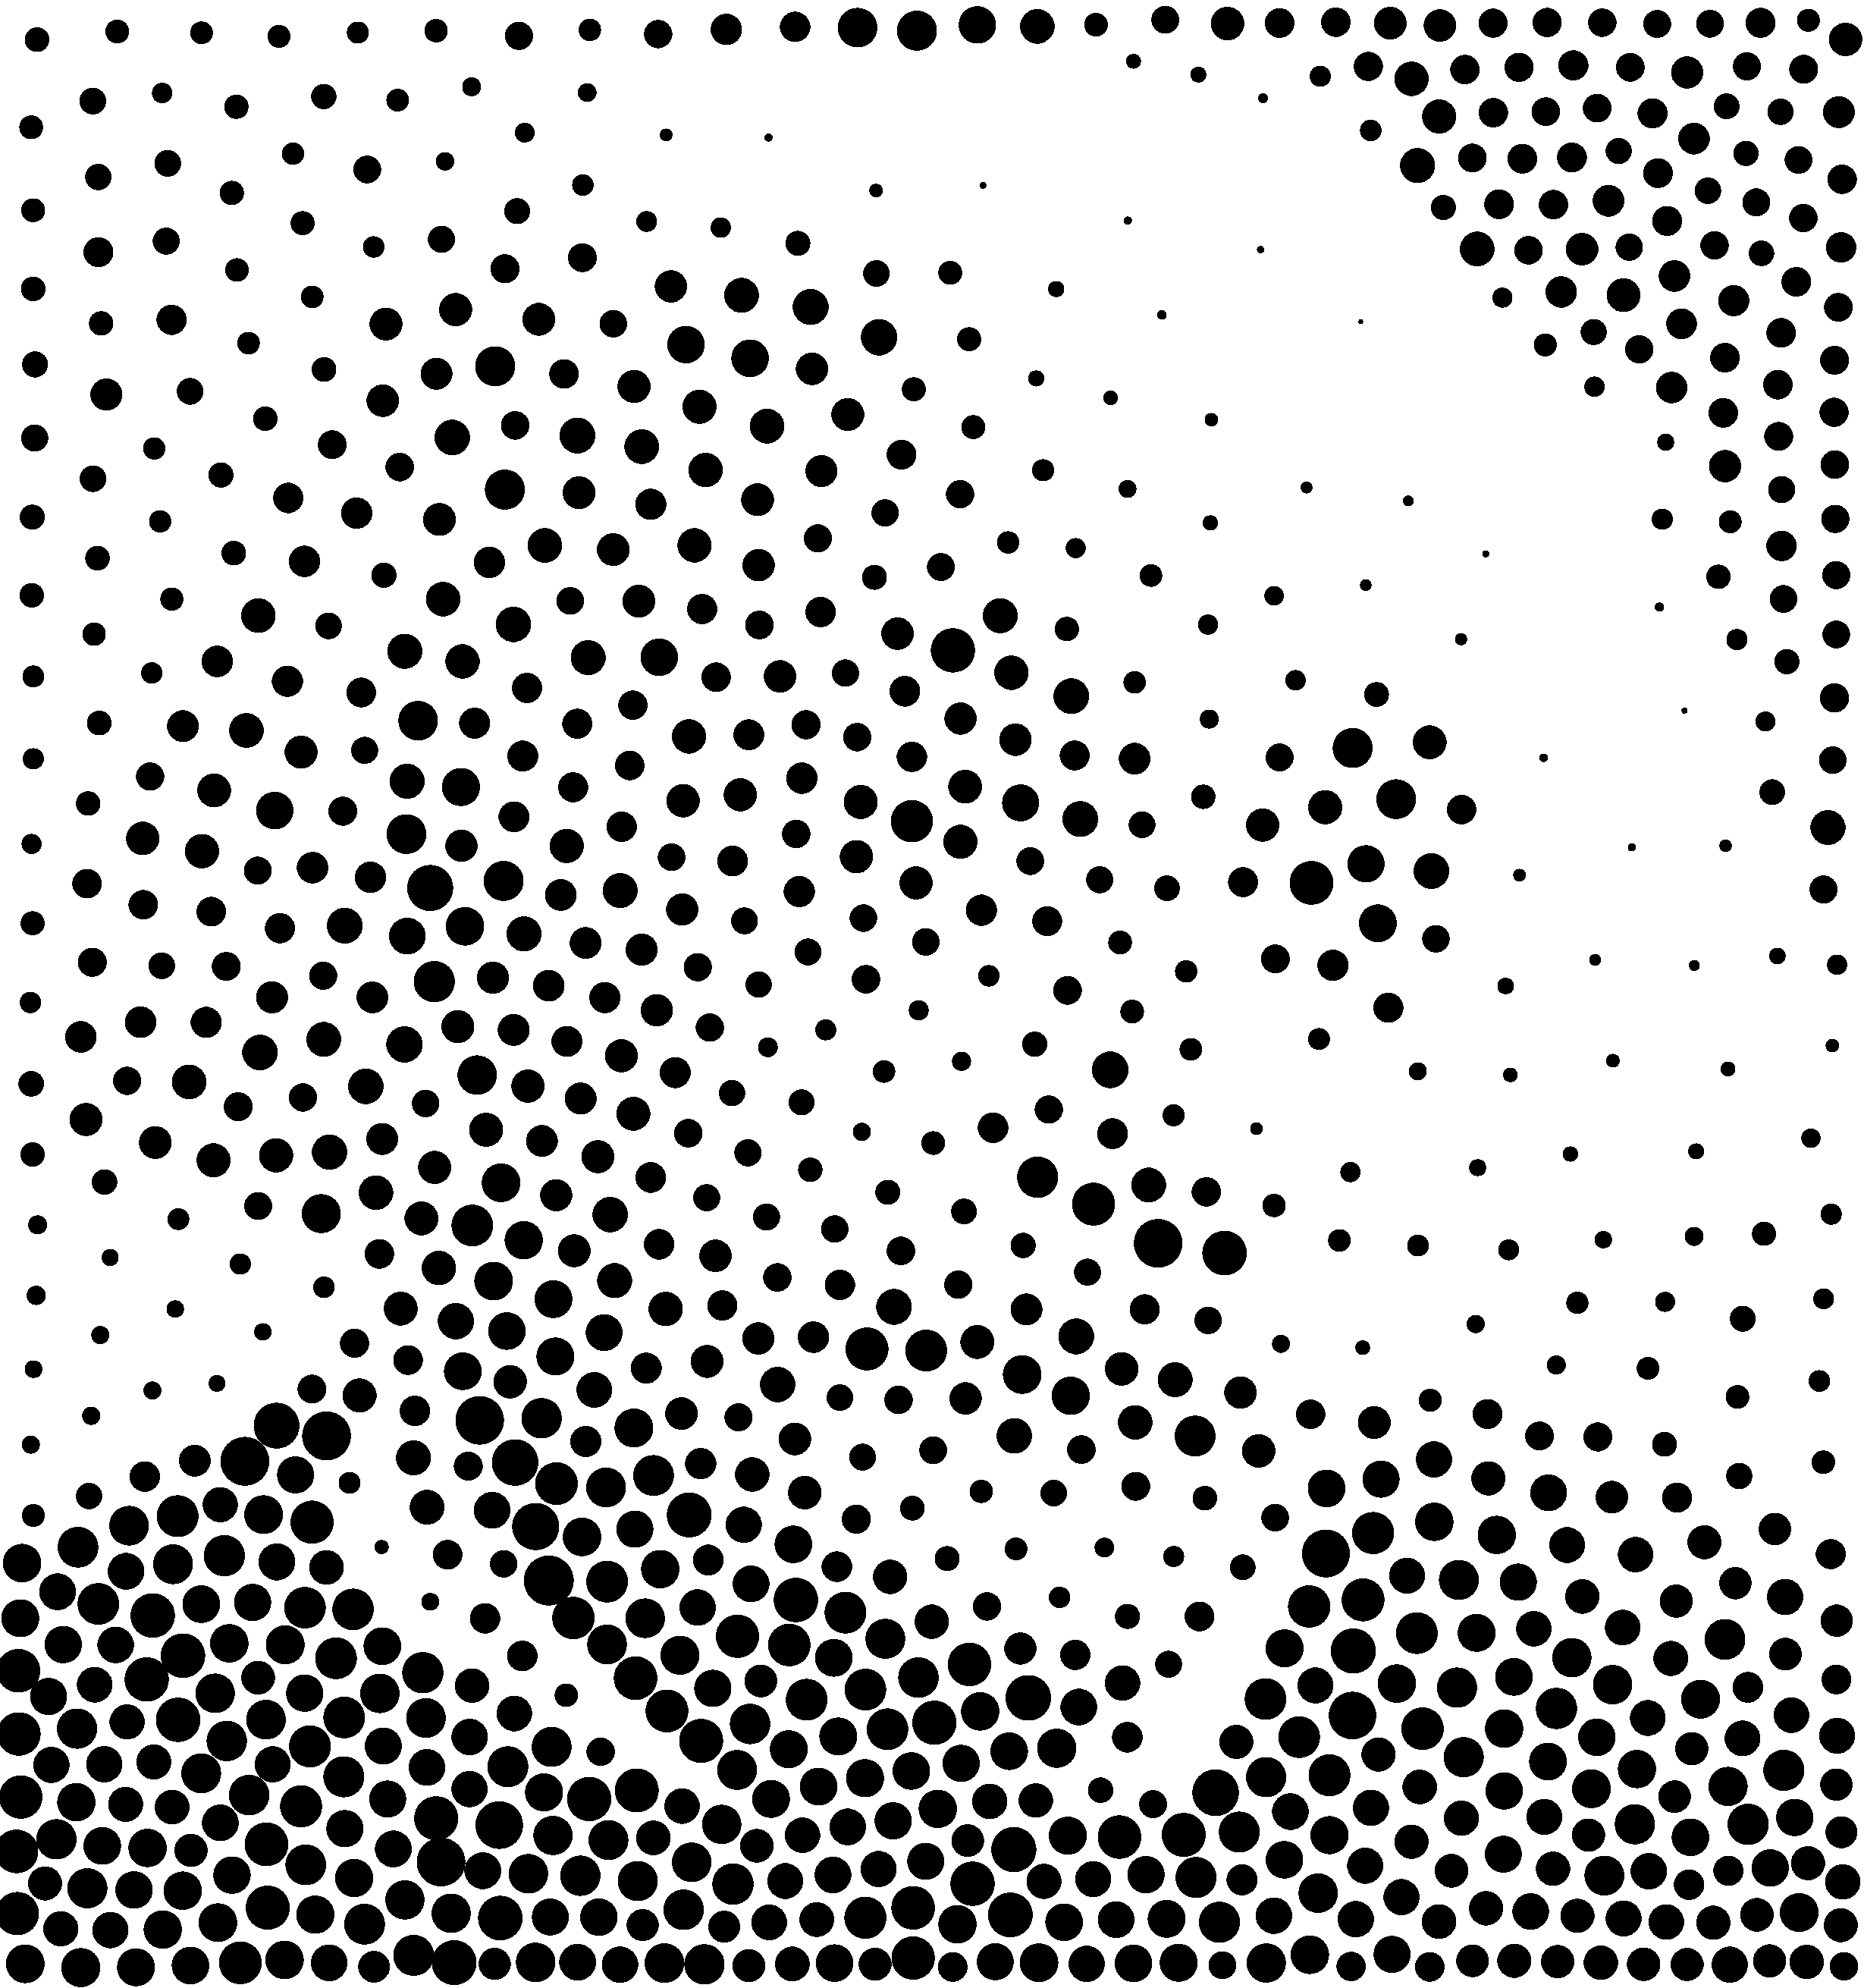
\includegraphics[width=\textwidth]{../results/voronoi/3-5.pdf}
 \caption{Large image size}
    \end{subfigure}
    \begin{subfigure}{0.4\textwidth}
        \centering
        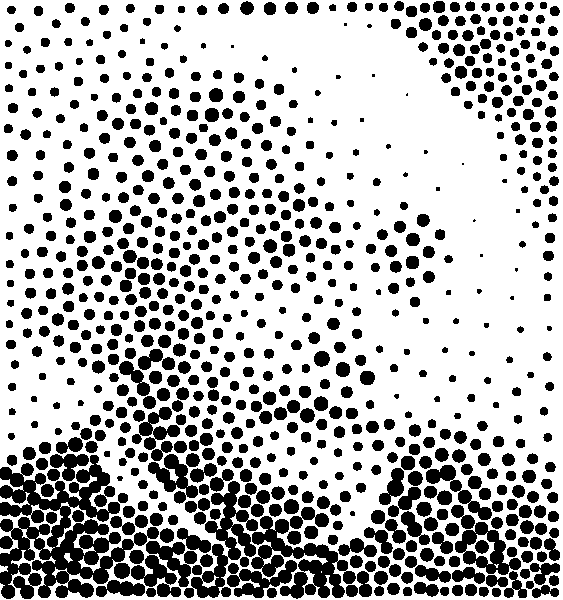
\includegraphics[width=\textwidth]{../results/voronoi/3-6.pdf}
 \caption{Small image size}
    \end{subfigure}
    \caption{Voronoi}
    \label{fig:2}
\end{figure}

The sizes of the images have great impact on the size of the radius of the disks generated using  hedcuter method, while  voronoi method is consistent  to the variance of image size. Because hedcuter calcuate the average intensity of the cell and this will impacted by the cell size, while voronoi uses the max intensity of the cell.

\begin{figure}[H]
    \centering
        \begin{subfigure}{0.4\textwidth}
        \centering
        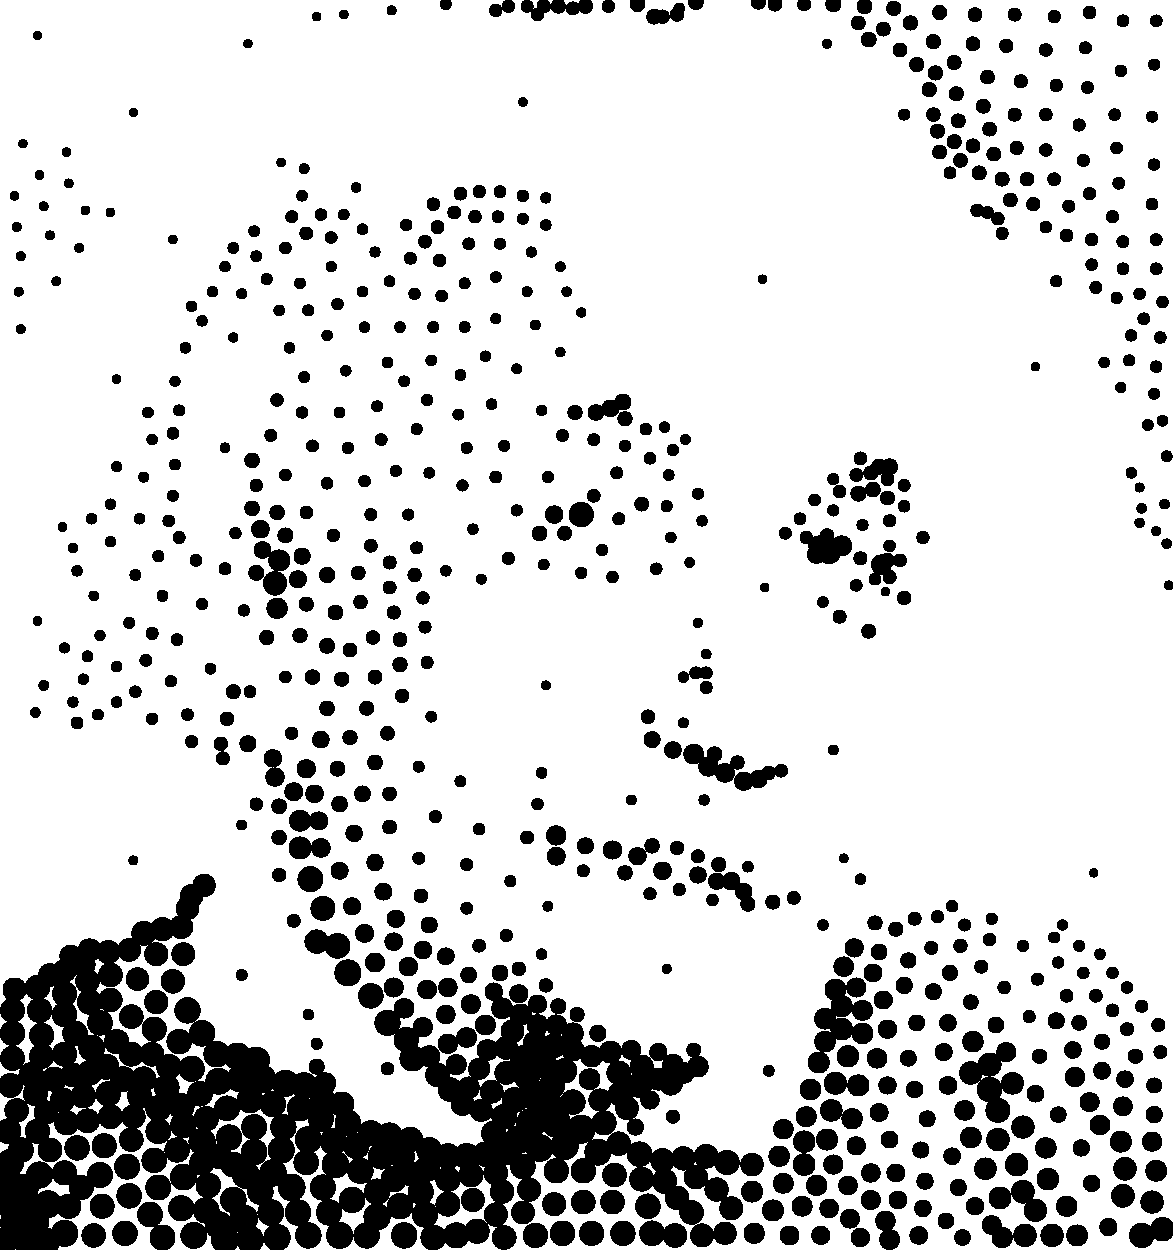
\includegraphics[width=\textwidth]{../results/hedcuter/3-3.pdf}
         \caption{High Brightness}
    \end{subfigure}
    \begin{subfigure}{0.4\textwidth}
        \centering
        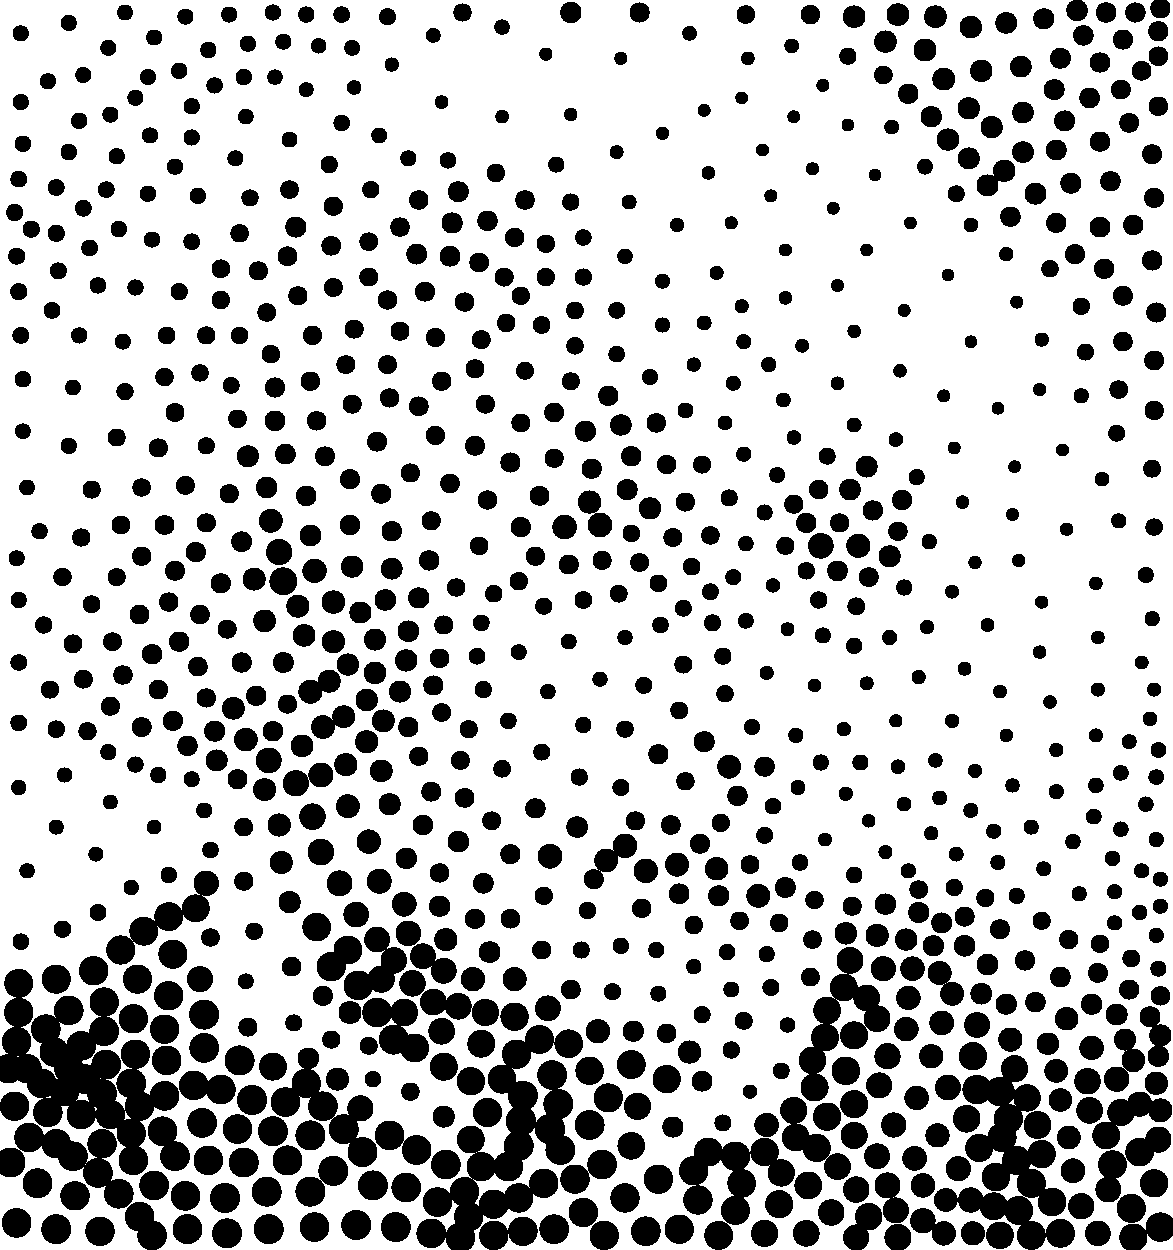
\includegraphics[width=\textwidth]{../results/hedcuter/3-4.pdf}
         \caption{Low Brightness}
    \end{subfigure}
    \label{fig:1}
        \caption{Hedcuter}
\end{figure}

\begin{figure}[H]
    \centering
        \begin{subfigure}{0.4\textwidth}
        \centering
        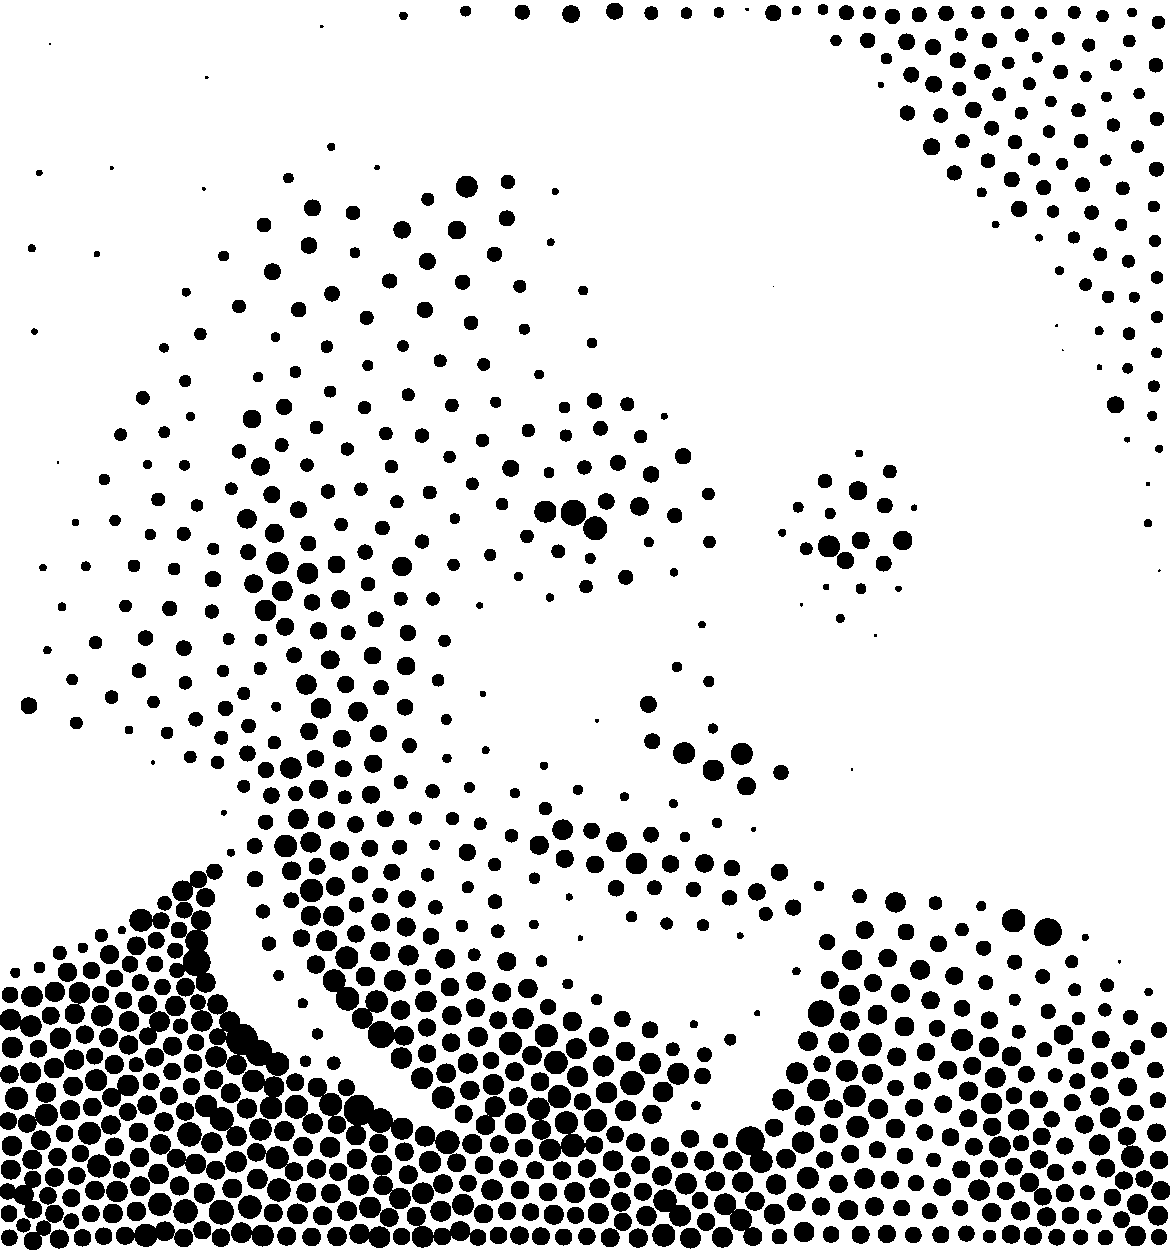
\includegraphics[width=\textwidth]{../results/voronoi/3-3.pdf}
 \caption{High Brightness}
    \end{subfigure}
    \begin{subfigure}{0.4\textwidth}
        \centering
        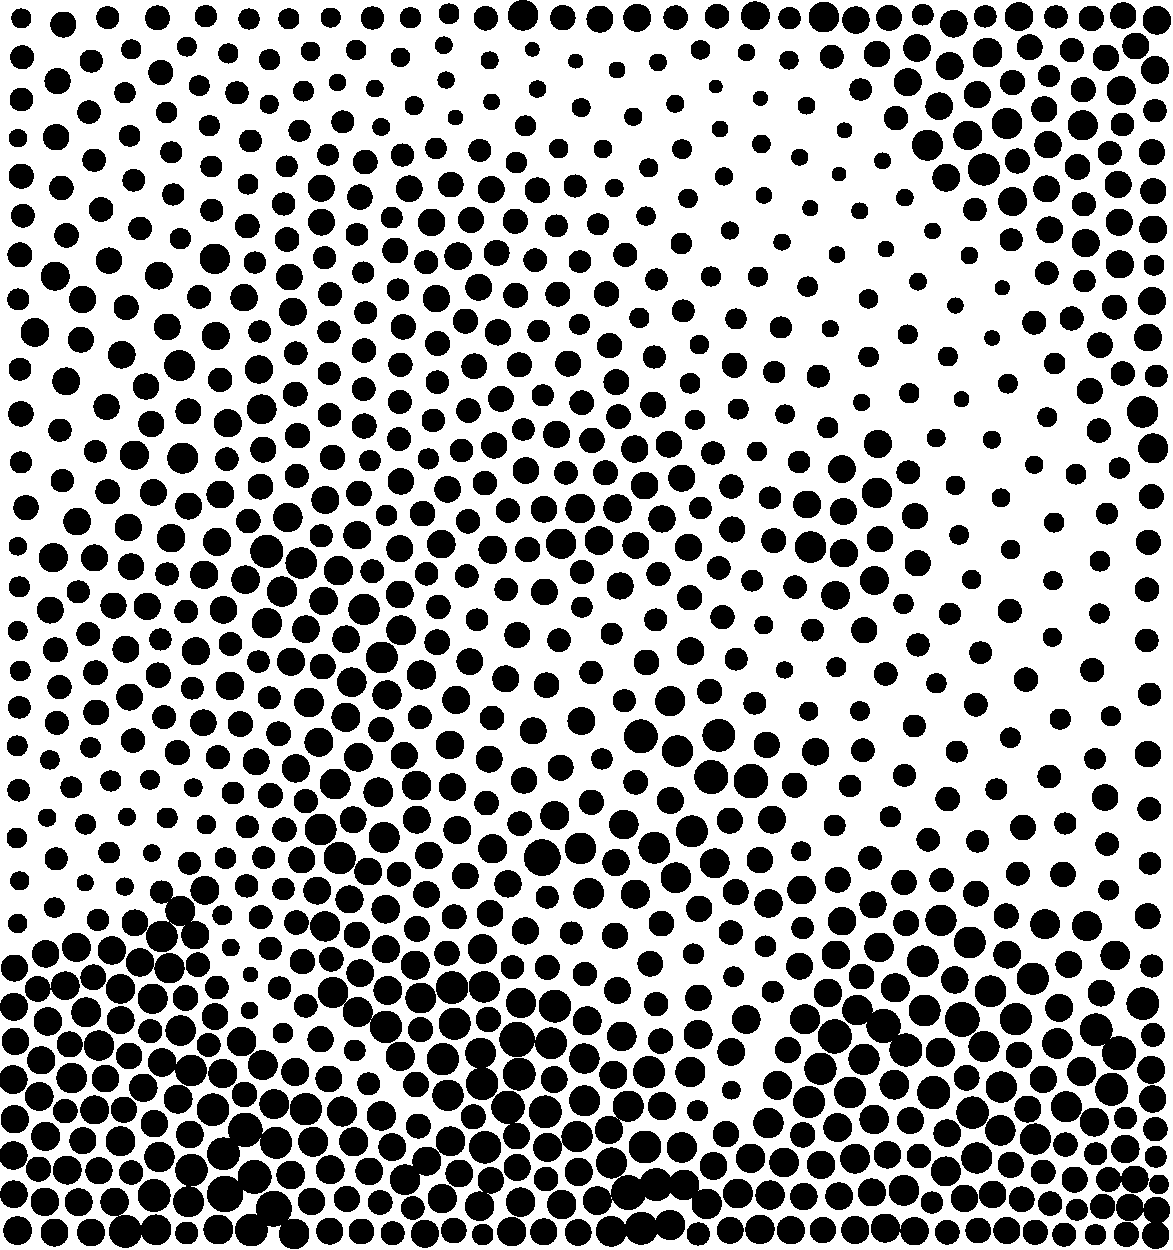
\includegraphics[width=\textwidth]{../results/voronoi/3-4.pdf}
 \caption{Low Brightness}
    \end{subfigure}
    \caption{Voronoi}
    \label{fig:2}
\end{figure}

Both methods are affected greatly by the brightness of the image, as the darker pixels prevail the image. However, the hedcuter seems maintain a better consistency due to the way it calculate the disk radius.

\begin{figure}[H]
    \centering
        \begin{subfigure}{0.4\textwidth}
        \centering
        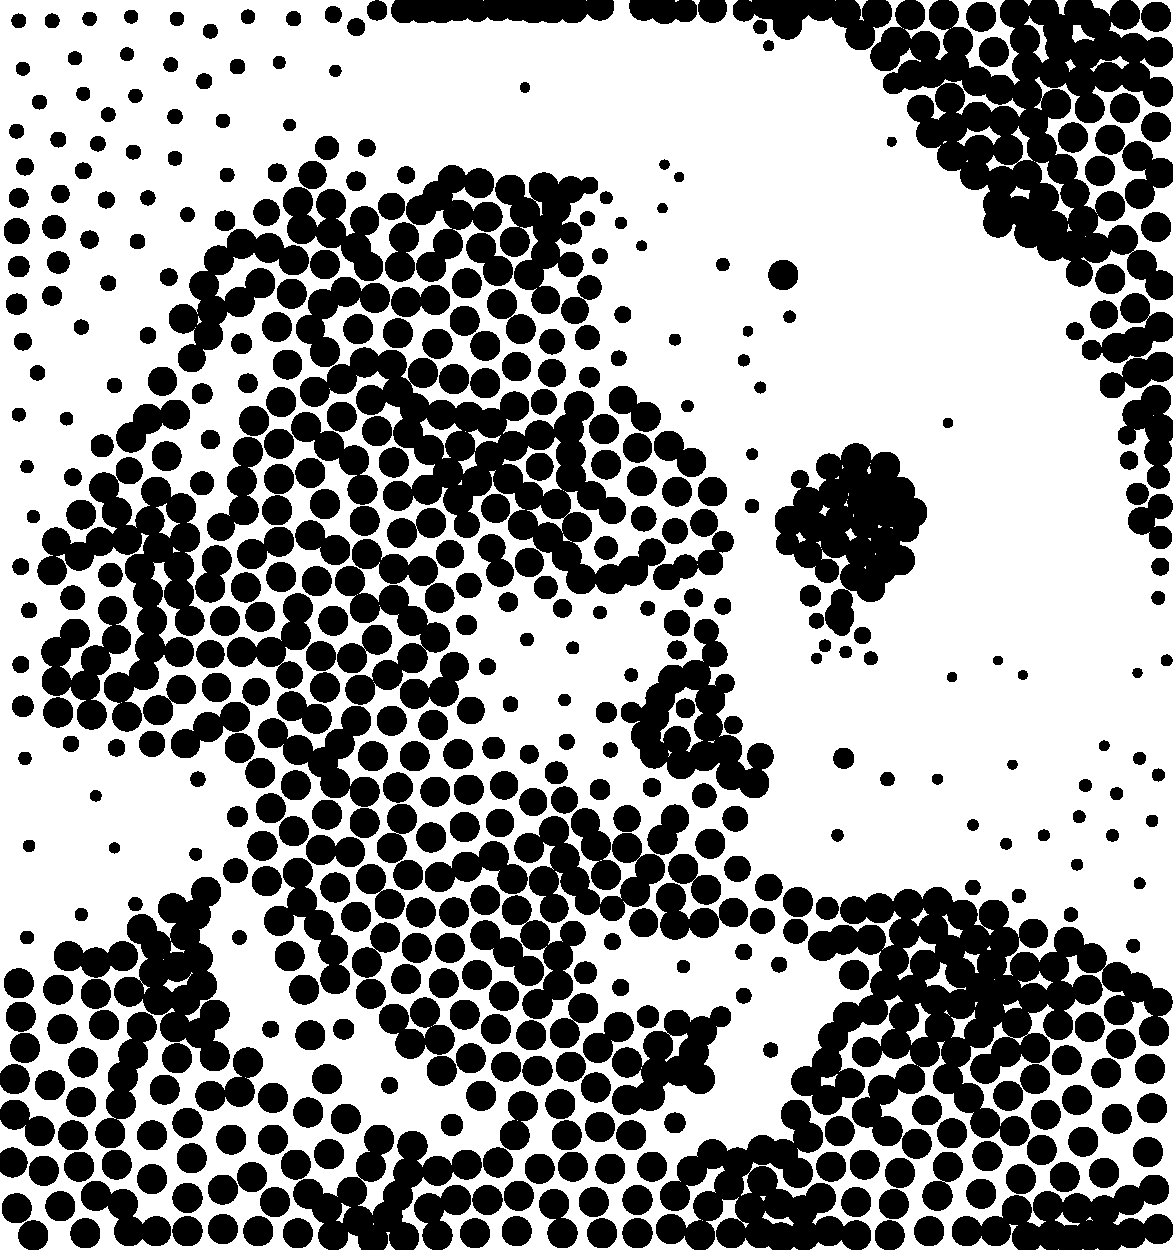
\includegraphics[width=\textwidth]{../results/hedcuter/3-1.pdf}
         \caption{High Contrast}
    \end{subfigure}
    \begin{subfigure}{0.4\textwidth}
        \centering
        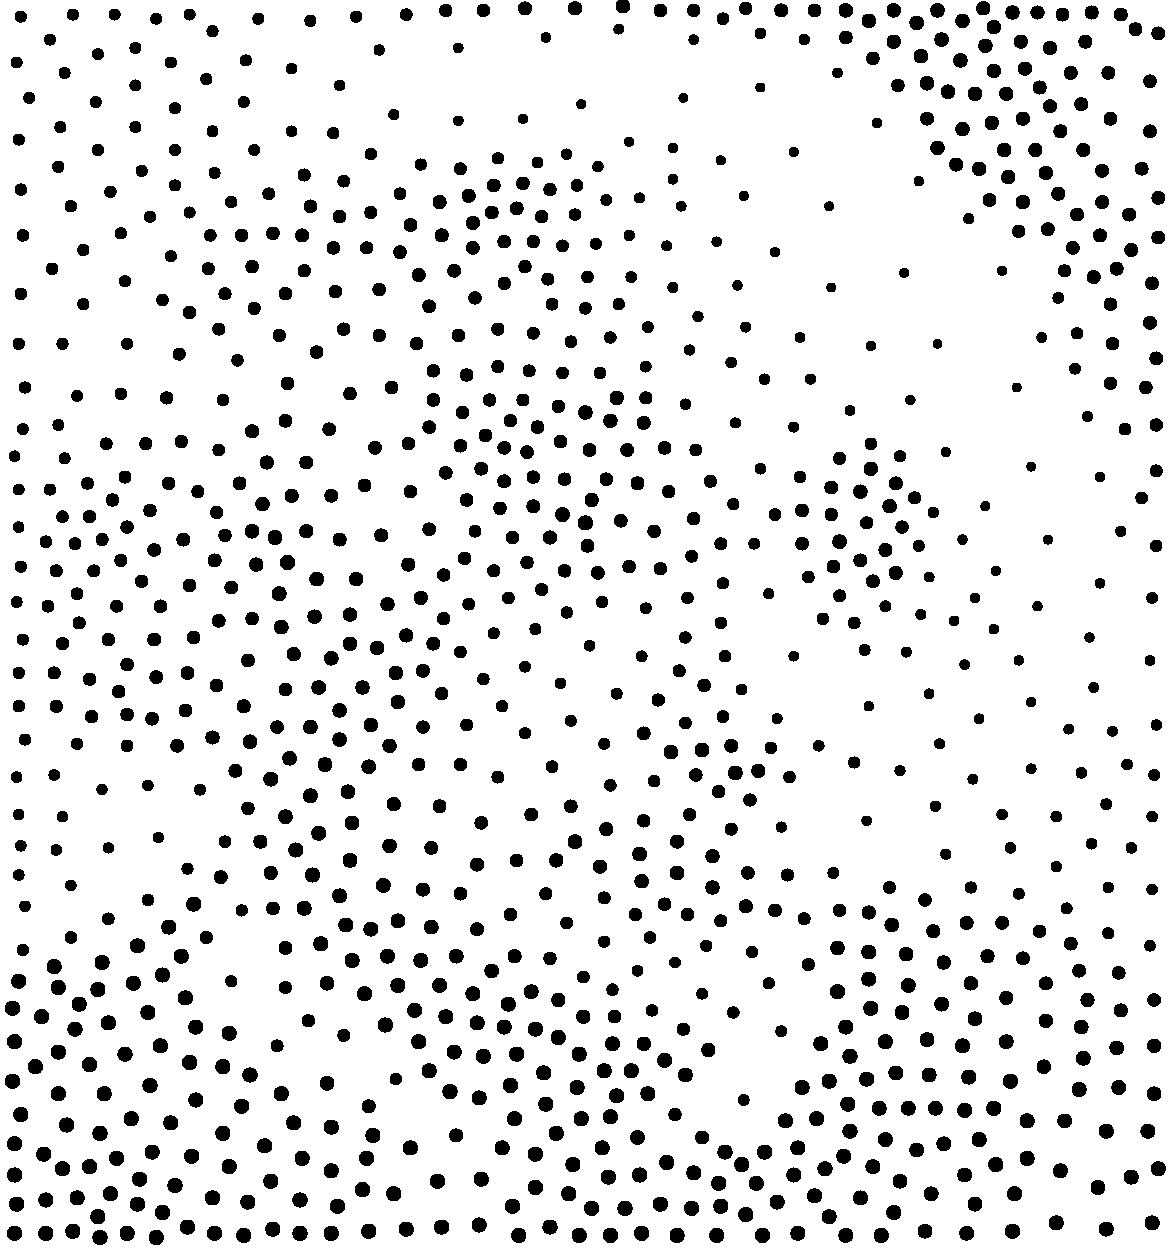
\includegraphics[width=\textwidth]{../results/hedcuter/3-2.pdf}
         \caption{Low Contrast}
    \end{subfigure}
    \label{fig:1}
        \caption{Hedcuter}
\end{figure}

\begin{figure}[H]
    \centering
        \begin{subfigure}{0.4\textwidth}
        \centering
        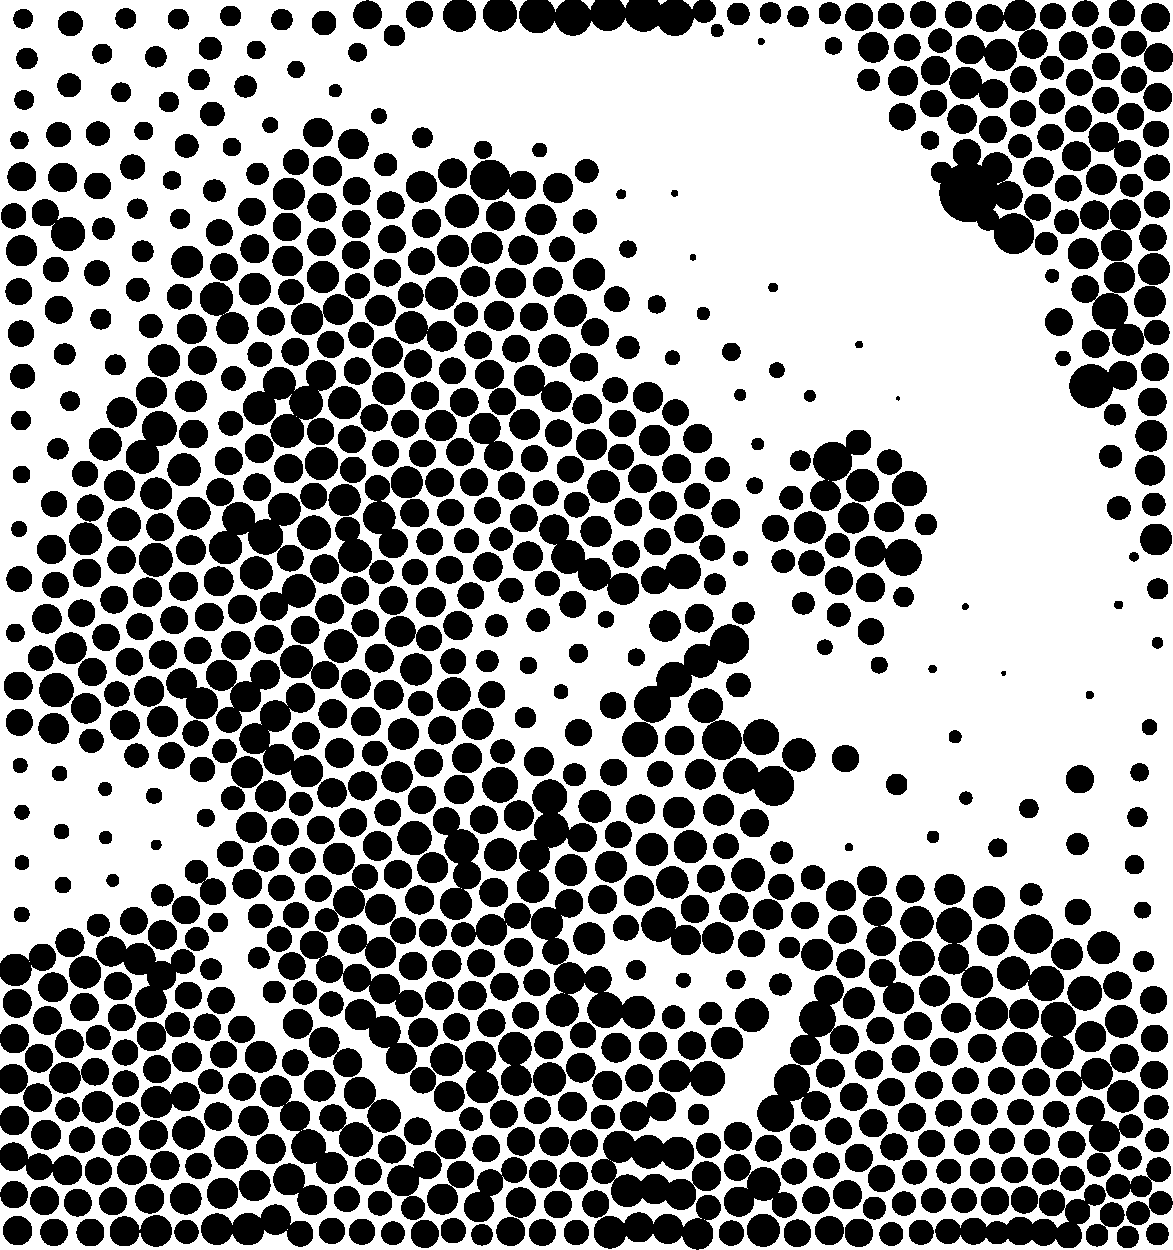
\includegraphics[width=\textwidth]{../results/voronoi/3-1.pdf}
 \caption{High Contrast}
    \end{subfigure}
    \begin{subfigure}{0.4\textwidth}
        \centering
        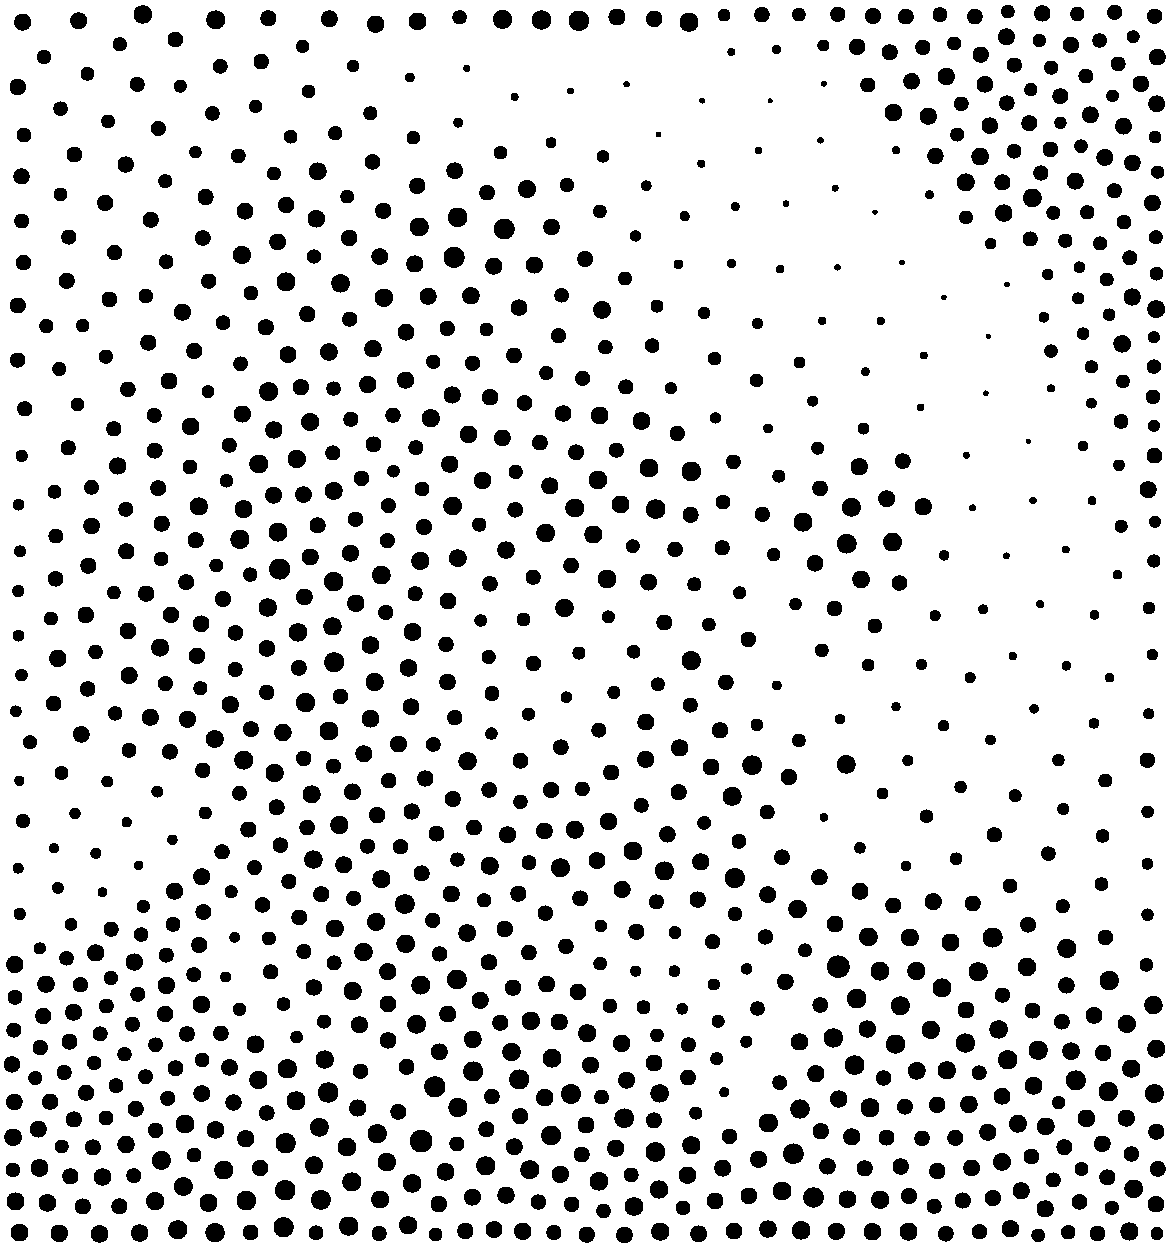
\includegraphics[width=\textwidth]{../results/voronoi/3-2.pdf}
 \caption{Low Contrast}
    \end{subfigure}
    \caption{Voronoi}
    \label{fig:2}
\end{figure}

Contrast is not a major factor that would increase of decrease the difference between the two methods.

\item Does the type of image (human vs. machine, natural vs. urban landscapes, photo vs. painting, etc) increase or decrease their difference?

\begin{figure}[H]
    \centering
        \begin{subfigure}{0.3\textwidth}
        \centering
        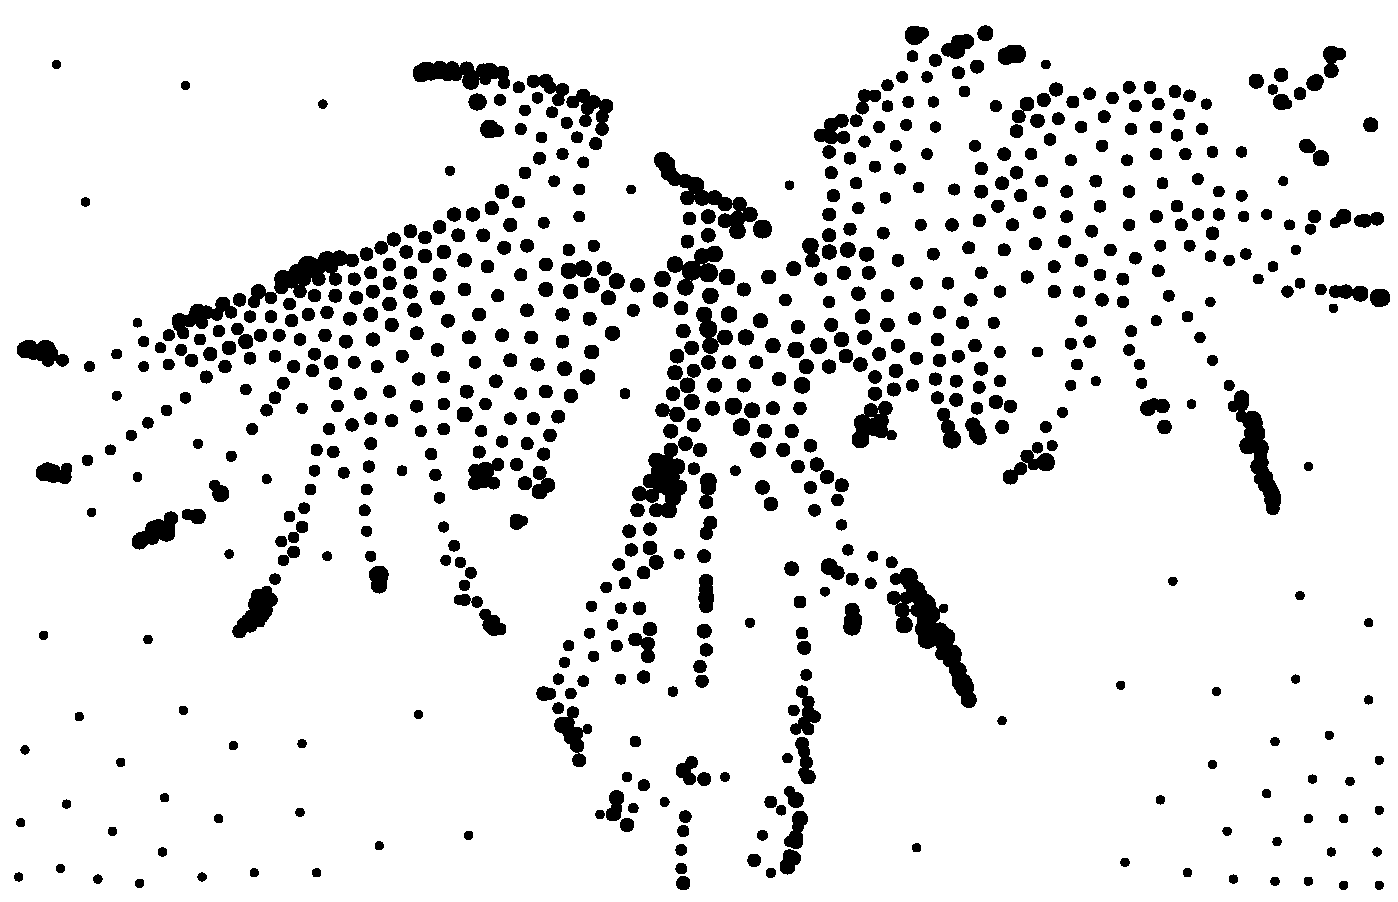
\includegraphics[width=\textwidth]{../results/hedcuter/4-1.pdf}
         \caption{Phoenix}
    \end{subfigure}
    \begin{subfigure}{0.3\textwidth}
        \centering
        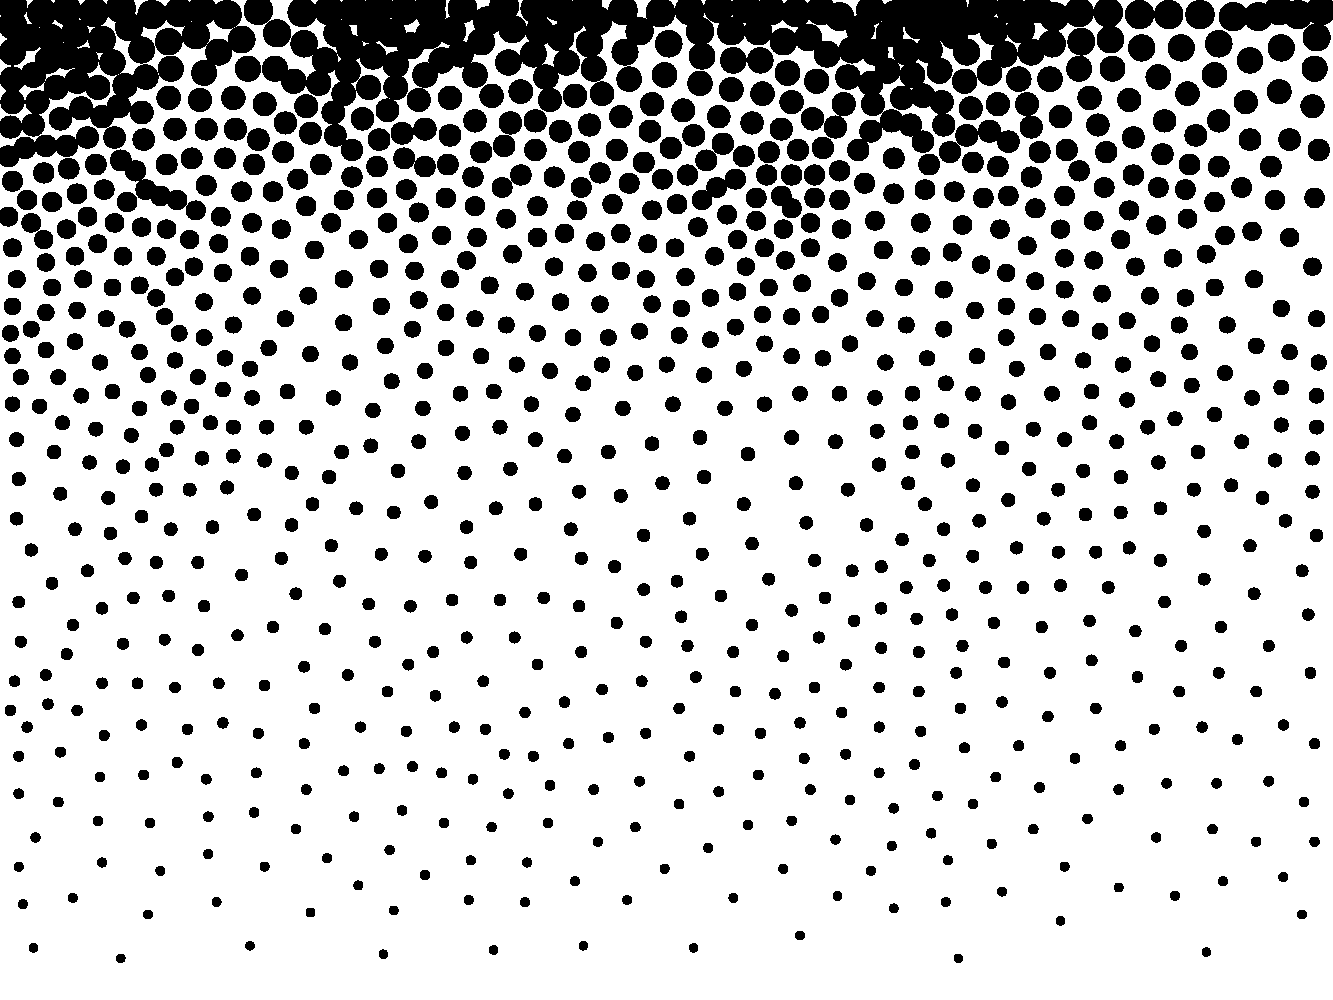
\includegraphics[width=\textwidth]{../results/hedcuter/4-2.pdf}
         \caption{Gradient}
    \end{subfigure}
        \begin{subfigure}{0.3\textwidth}
        \centering
        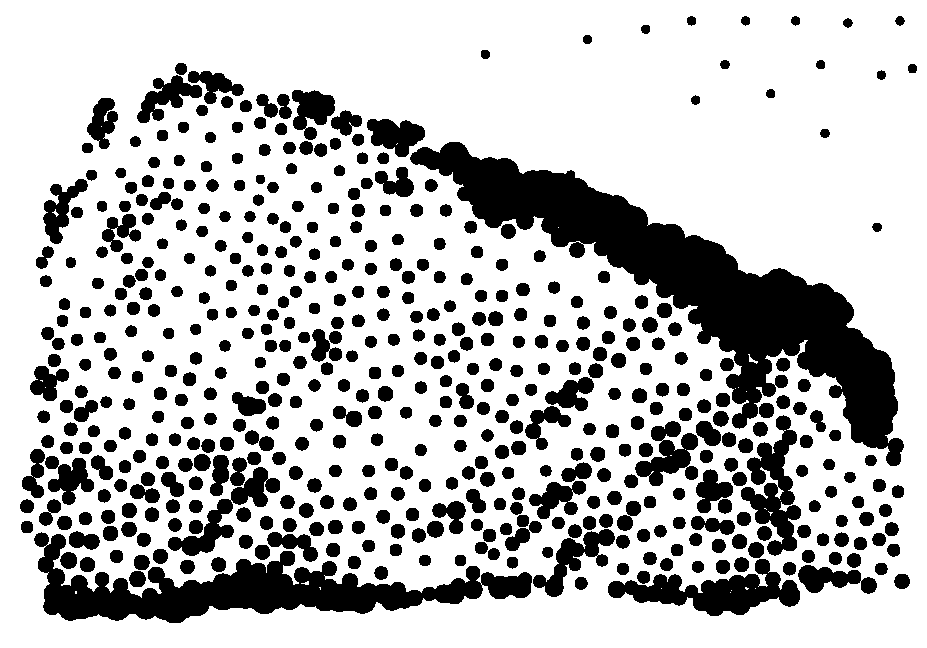
\includegraphics[width=\textwidth]{../results/hedcuter/4-3.pdf}
         \caption{Erinking}
    \end{subfigure}
        \caption{Hedcuter}
            \label{fig:type_h}
\end{figure}

\begin{figure}[H]
    \centering
        \begin{subfigure}{0.3\textwidth}
        \centering
        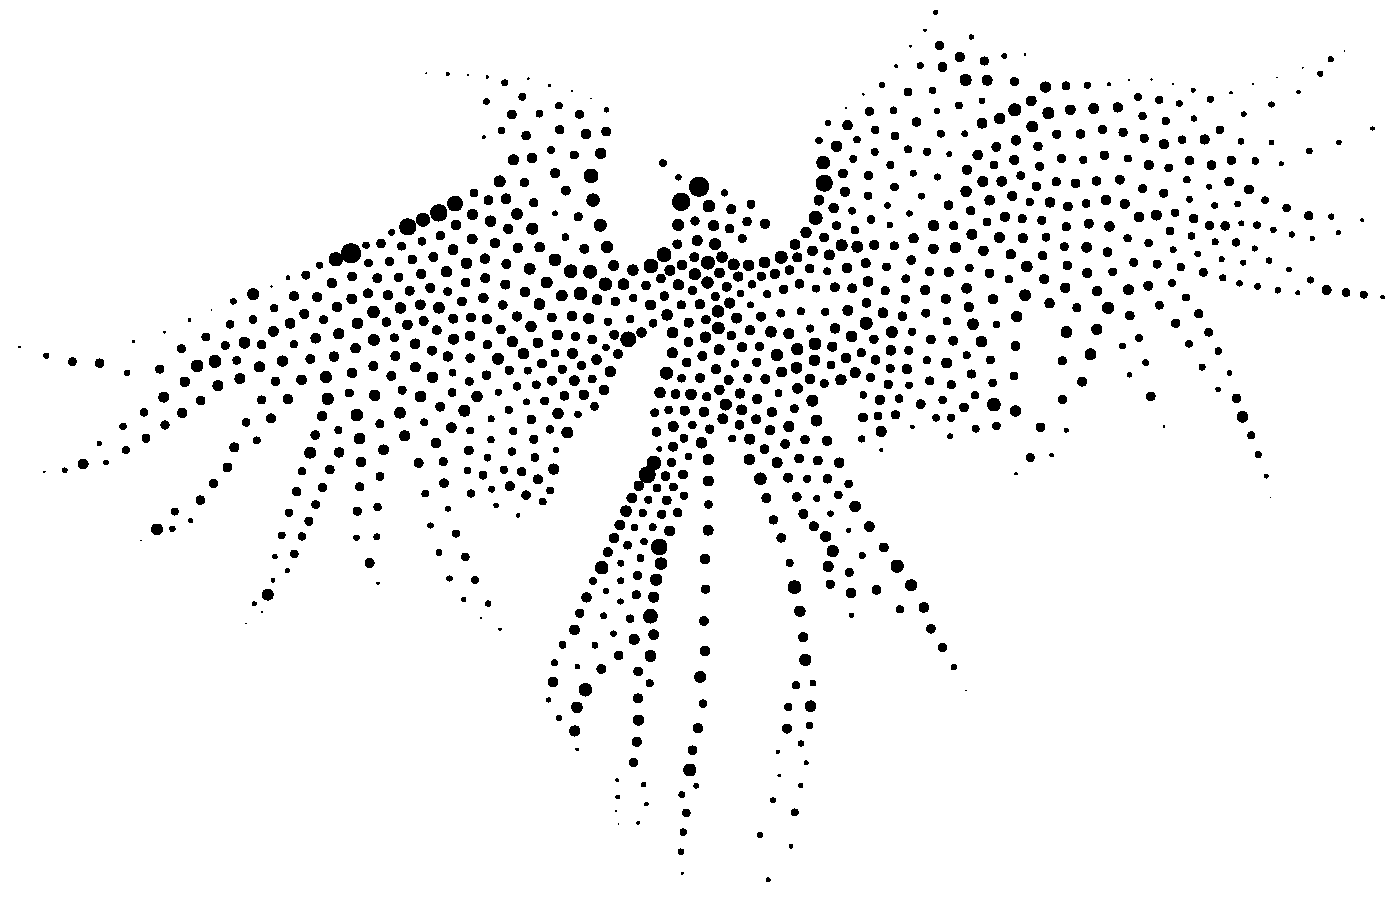
\includegraphics[width=\textwidth]{../results/voronoi/4-1.pdf}
 \caption{Phoenix}
    \end{subfigure}
    \begin{subfigure}{0.3\textwidth}
        \centering
        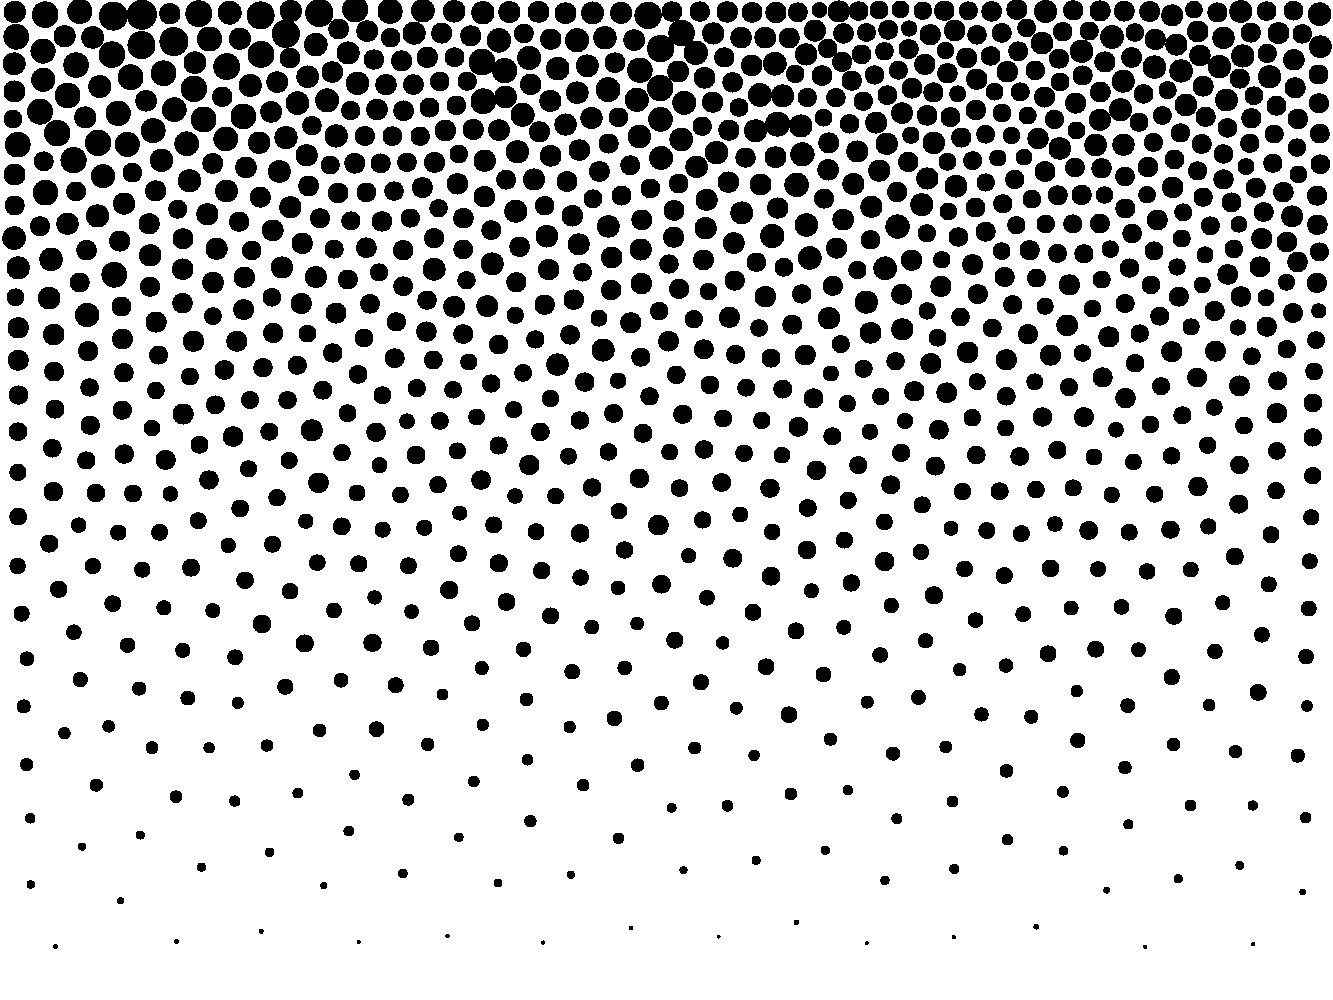
\includegraphics[width=\textwidth]{../results/voronoi/4-2.pdf}
 \caption{Gradient}
    \end{subfigure}
    \begin{subfigure}{0.3\textwidth}
        \centering
        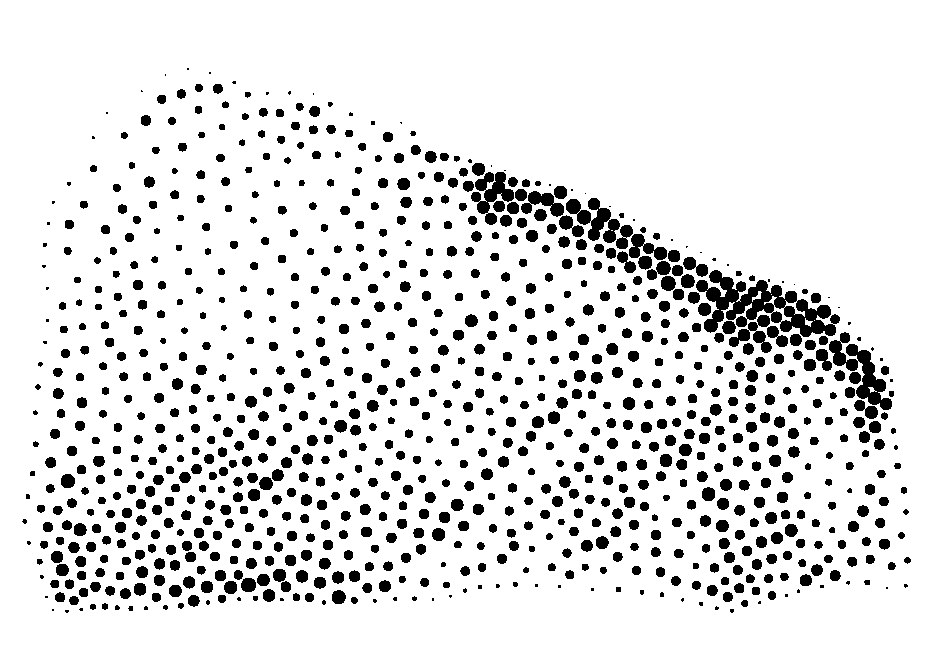
\includegraphics[width=\textwidth]{../results/voronoi/4-3.pdf}
 \caption{Erinking}
    \end{subfigure}
    \caption{Voronoi}
    \label{fig:type_v}
\end{figure}

Based the observation on \ref{fig:type_h} and \ref{fig:type_v}, different subjects in the image does not have much effect on the performance of the two methods.

\item Are the outputs of these stippling methods different the hedcut images created by artists (e.g. those from the Wall Street Journal)?

\begin{figure}[H]
    \centering
     \begin{subfigure}{0.4\textwidth}
        \centering
        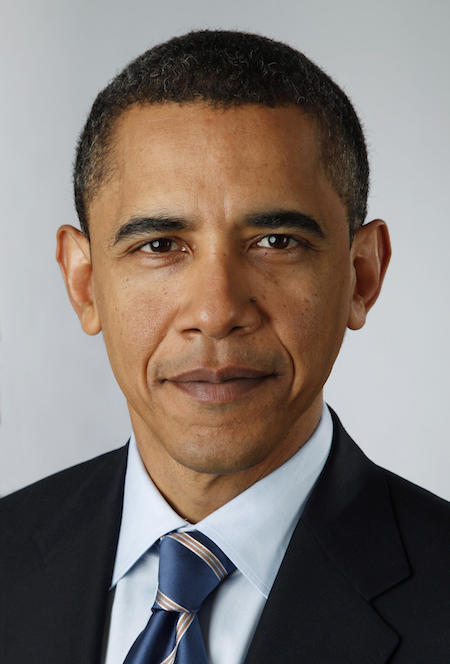
\includegraphics[width=\textwidth]{../images/obama.png}
 \caption{Photo}
    \end{subfigure}
        \begin{subfigure}{0.4\textwidth}
        \centering
        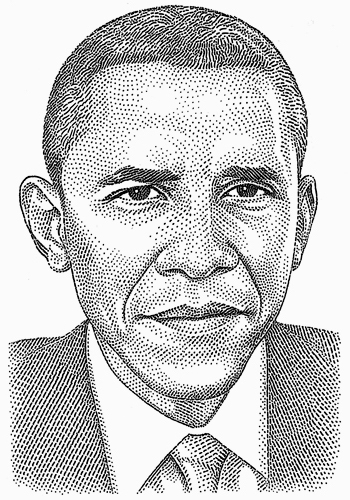
\includegraphics[width=\textwidth]{figs/wsj-obama.jpg}
 \caption{WSJ artist stippling}
    \end{subfigure}
    \begin{subfigure}{0.4\textwidth}
        \centering
        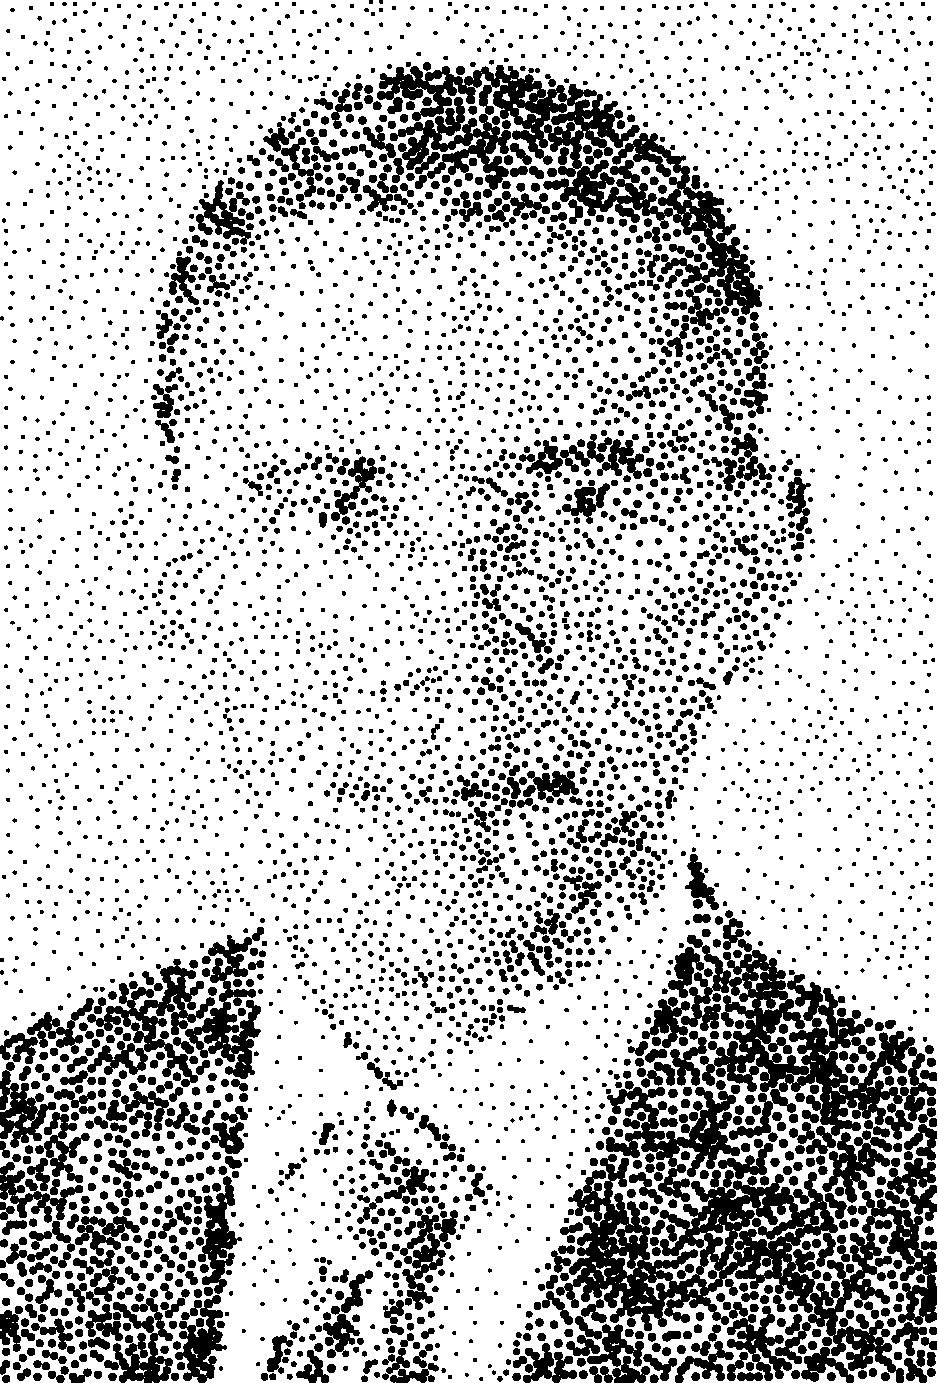
\includegraphics[width=\textwidth]{../results/hedcuter/5-1.pdf}
 \caption{Hedcuter}
    \end{subfigure}
    \begin{subfigure}{0.4\textwidth}
        \centering
        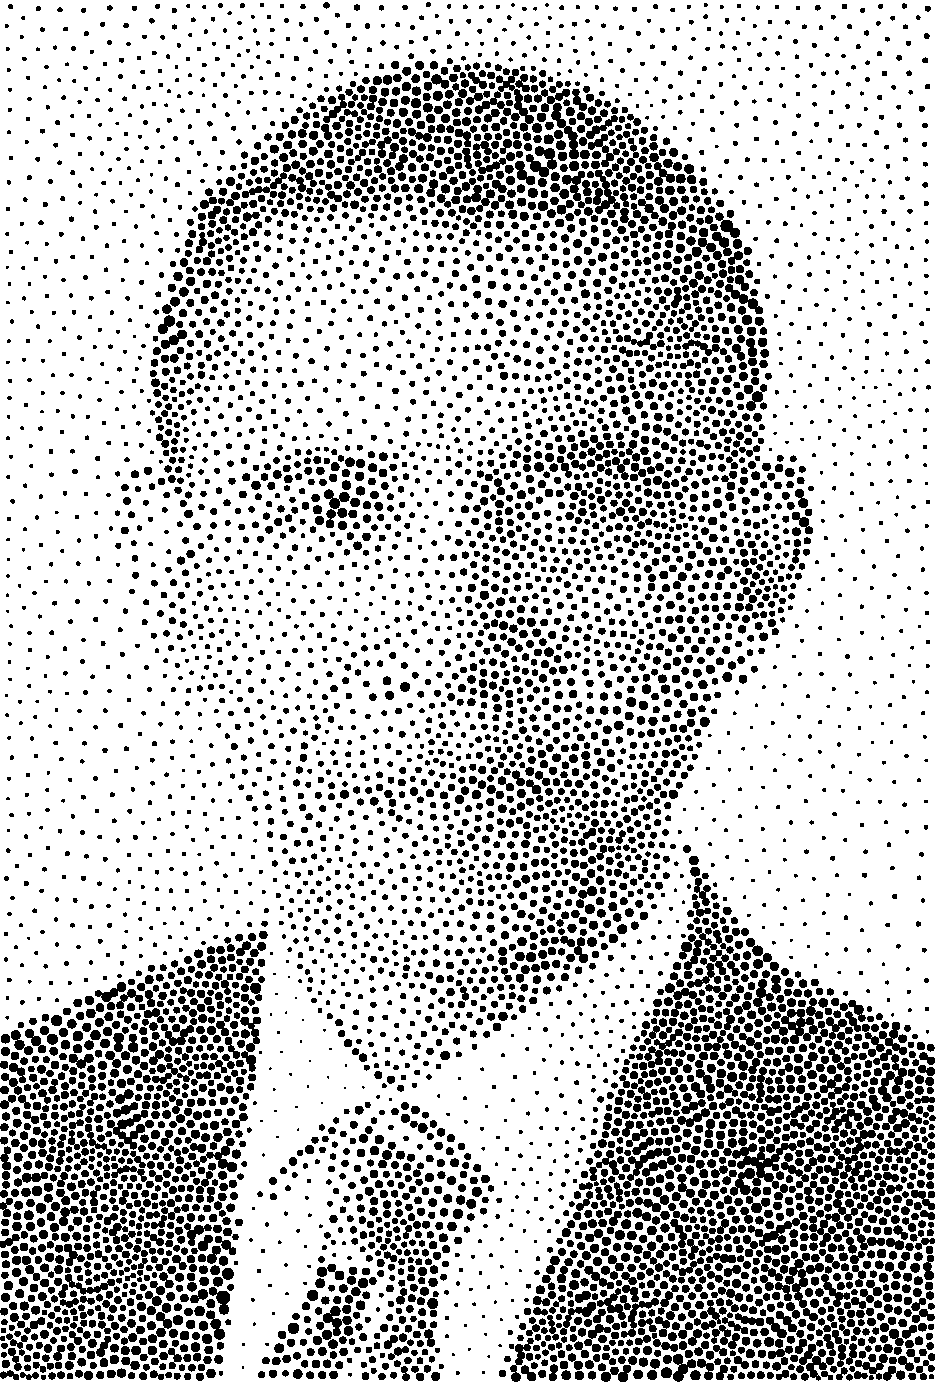
\includegraphics[width=\textwidth]{../results/voronoi/5-1.pdf}
 \caption{Voronoi}
    \end{subfigure}
    \caption{Comparison of WSJ artist stippling vs outputs of these stippling methods.}
    \label{fig:art}
\end{figure}

Clearly, both methods cannot create a stippling on par with the human art work, especially the the distribution of dots. The artist will strengthen the edge of the object and the stippling shows better contrast. These are all based on the semantic understanding of the object. The computer generated is pure base on each independent pixels and has nothing to do with the semantics.

\end{enumerate}

\section{Improvement of hedcuter method}

\subsection*{Improvement 1: Weighted Coloring}
The ideas is the pixel the centroid has larger weight in  determining the color of the disk than the pixels around the boundary.
I employed  the following weighted method to improve coloring in Algorithm \ref{alg:st_hed} Line 4.
$$d.rgb =\frac{\sum_{p \in c.P} {\xi_p \cdot M(p)} } {\sum{\xi_p}}$$
where 
\begin{eqnarray*}
\xi_p
\begin{cases}
1, & \text{if } p = p_c\cr 
\frac{1}{ \text{euclidean\_dist}(p,p_c)  }, & \text{otherwise} \cr
\end{cases}
\end{eqnarray*}
given $p_c$ is the centroid of the cell containing $p$.

\begin{figure}[H]
    \centering
            \begin{subfigure}{0.4\textwidth}
        \centering
        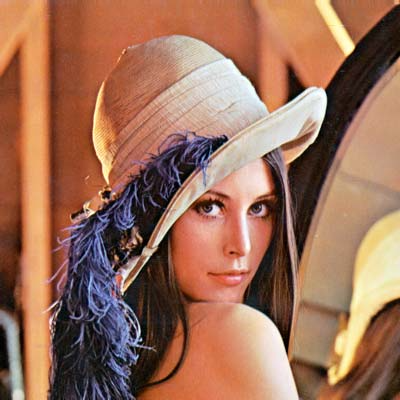
\includegraphics[width=\textwidth]{../images/lenna.png}
 \caption{Input image: Lenna}
    \end{subfigure}
    \begin{subfigure}{0.4\textwidth}
        \centering
        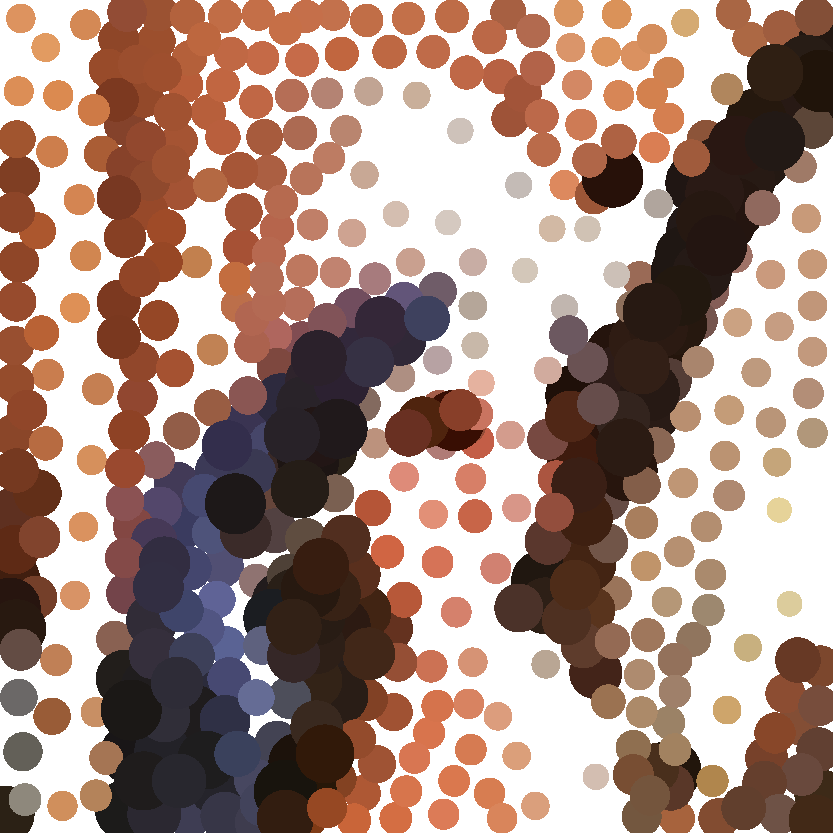
\includegraphics[width=\textwidth]{../results/hedcuter/A-1.pdf}
 \caption{Disk color based on cell average}
    \end{subfigure}
        \begin{subfigure}{0.4\textwidth}
        \centering
        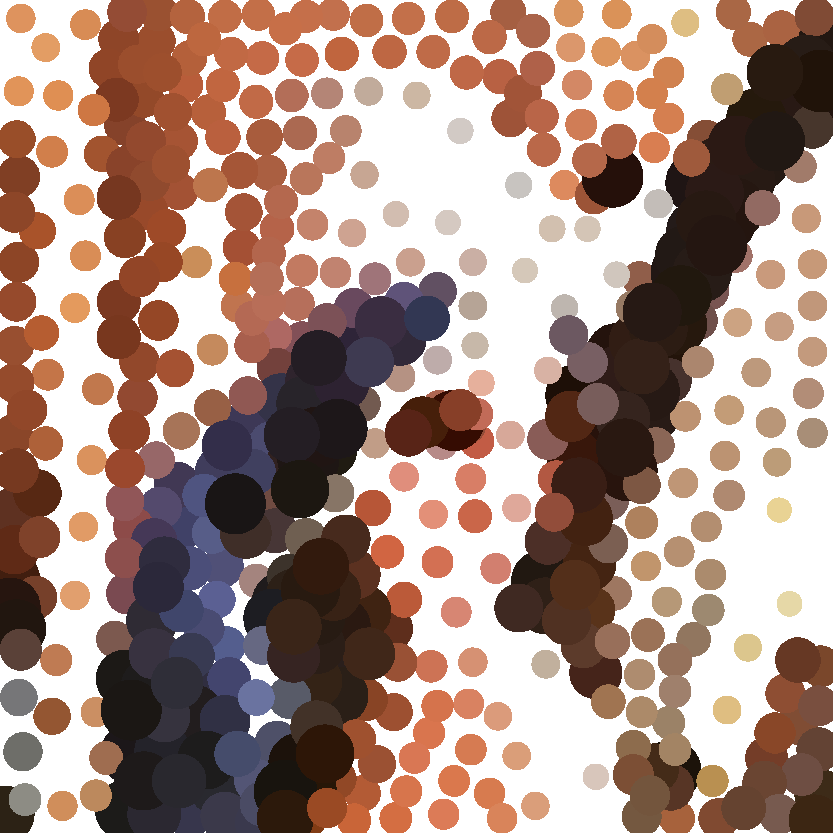
\includegraphics[width=\textwidth]{../results/hedcuter/A-2.pdf}
 \caption{Disk color based on  weighted cell average}
    \end{subfigure}
    \begin{subfigure}{0.4\textwidth}
        \centering
        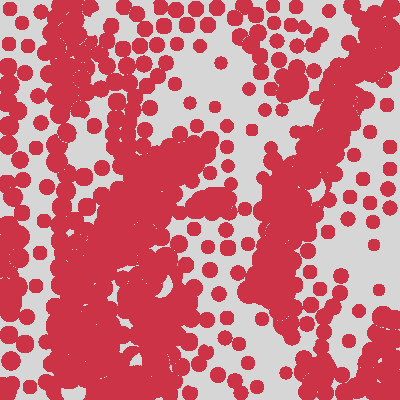
\includegraphics[width=\textwidth]{../results/hedcuter/A-3.png}
 \caption{Difference of (b) and (c)}
    \end{subfigure}
    \caption{Comparison of color based on average cell color vs. weight average cell color. }
    \label{fig:color}
\end{figure}

The results are shown in Figure \ref{fig:color}, depending on the monitor, the color enhancement might be hard to tell. The different area of the two output are shown in \ref{fig:color} (d).

\subsection*{Improvement 2: Disk Radius Based on Cell Area}
I employed  the following weighted method to improve coloring in Algorithm \ref{alg:st_hed} Line 6.
$$d.r =\frac{ r\cdot \text{area}(c) } { \max_{c \in C}{(\text{area}(c) )}}$$

The results are shown in Figure \ref{fig:radius}

\begin{figure}[H]
    \centering
        \begin{subfigure}{0.4\textwidth}
        \centering
        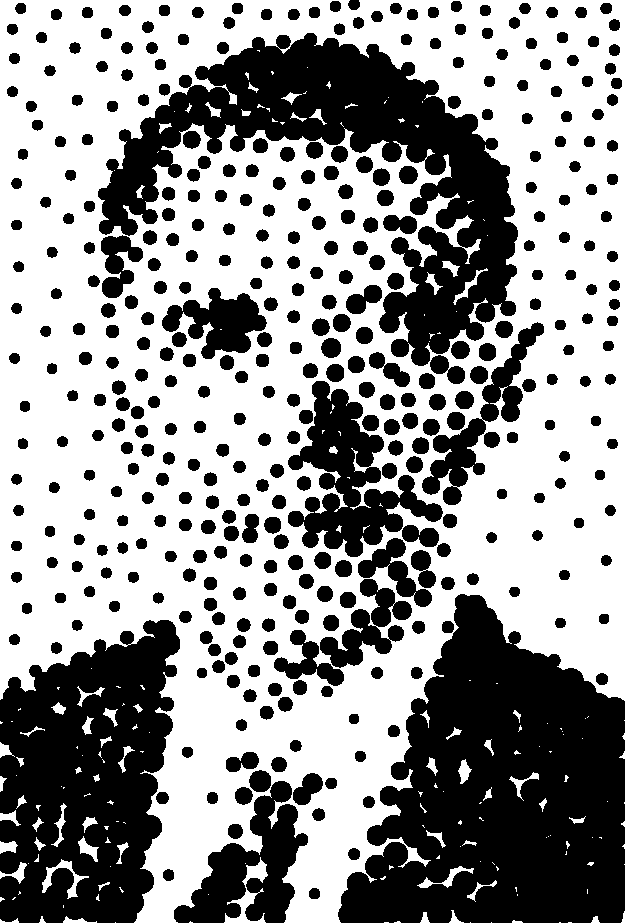
\includegraphics[width=\textwidth]{../results/hedcuter/B-1.pdf}
 \caption{Disk radius based on intensity}
    \end{subfigure}
    \begin{subfigure}{0.4\textwidth}
        \centering
        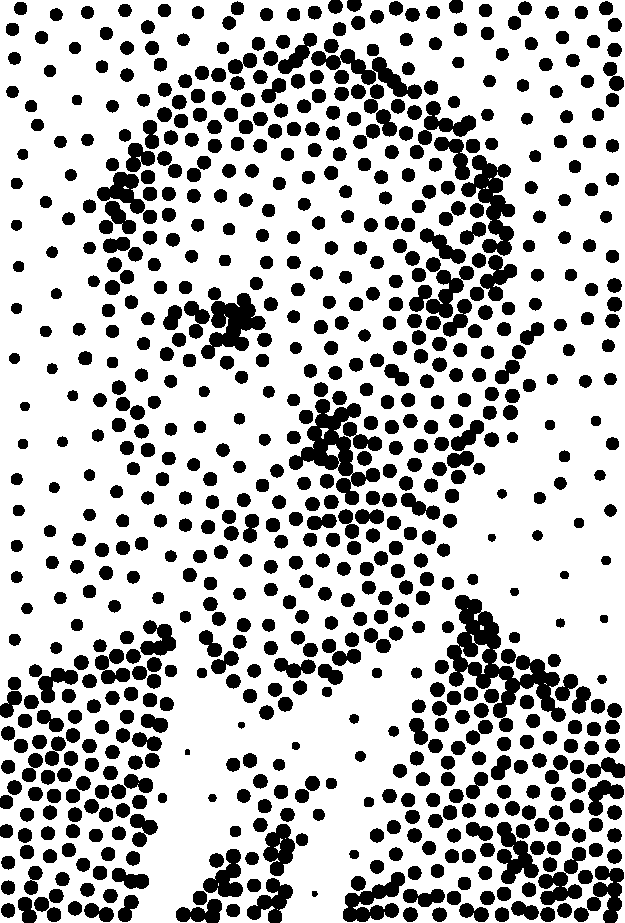
\includegraphics[width=\textwidth]{../results/hedcuter/B-2.pdf}
 \caption{Disk radius based on cell area}
    \end{subfigure}
    \caption{Comparison of disk radius based on intensity vs. disk radius based on cell area}
    \label{fig:radius}
\end{figure}



\subsection*{Improvement 3: Stippling Reconstruction}

The idea is that we can obtain a stippling image created by artist, like the Wall Street Journal ones that are printed on a piece of paper, then we digitize it by extracting the stippling points $(x,y)$ locations from a scanned copy. If we reconstruct a existing stippling, we can recreate many things like re-coloring based on an existing art work. 

I implemented this functionality in the following step
\begin{enumerate}
\item collect all dark pixels in the scanned stippling (greyscale) image.
\item run a Density-based spatial clustering of applications with noise (DBSCAN)\cite{ester} on the extracted pixels locations, so that in the original image many dark pixels from the same disk are joined into one site.
\item build a voronoi diagram on  the sites obtained in the previous step.
\end{enumerate}

To show the result, I reconstructed a black and white stippling image and recolored it based on the reconstruction and the original photo. The results are shown in Figure \ref{fig:rec} It is very difficult to obtain the original photo of a artist created stippling, so I just use voronoi method to generate a stippling then printed it in a image.

\begin{figure}[H]
    \centering
            \begin{subfigure}{0.3\textwidth}
        \centering
        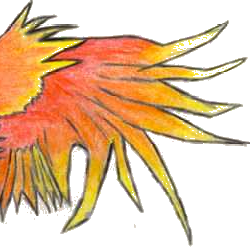
\includegraphics[width=\textwidth]{../images/phoenix_small.png}
 \caption{Input photo}
    \end{subfigure}
        \begin{subfigure}{0.3\textwidth}
        \centering
        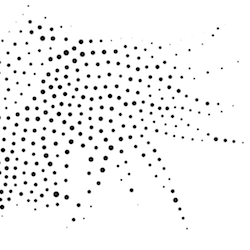
\includegraphics[width=\textwidth]{../images/phoenix_stipple_small.png}
 \caption{Input stippling image of (a)}
    \end{subfigure}
    \begin{subfigure}{0.3\textwidth}
        \centering
        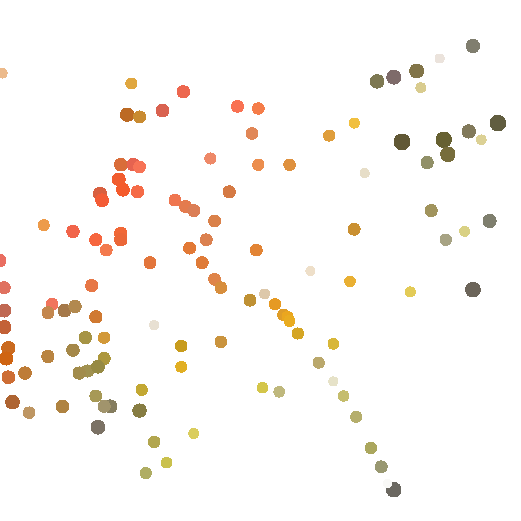
\includegraphics[width=\textwidth]{../results/hedcuter/C-1.pdf}
 \caption{Output of reconstructed stippling}
    \end{subfigure}
    \caption{Stippling reconstruction}
    \label{fig:rec}
\end{figure}

\section{Known Bugs and Limitations}

The stippling reconstruction only works for small number of stippling points, mainly due to the computational complexity of the DBSCAN clustering algorithm.

\bibliographystyle{plain}
\begin{thebibliography}{9}
\bibitem{secord} 
Adrian Secord. 2002. Weighted Voronoi stippling. In Proceedings of the 2nd international symposium on Non-photorealistic animation and rendering (NPAR '02). ACM, New York, NY, USA, 37-43.

\bibitem{ester}
Martin Ester, Hans-Peter Kriegel, Jörg Sander, and Xiaowei Xu. 1996. A density-based algorithm for discovering clusters a density-based algorithm for discovering clusters in large spatial databases with noise. In Proceedings of the Second International Conference on Knowledge Discovery and Data Mining (KDD'96), Evangelos Simoudis, Jiawei Han, and Usama Fayyad (Eds.). AAAI Press 226-231.

\end{thebibliography}


\end{document}


